\documentclass{article}
\usepackage{float}
\usepackage{graphicx} % Required for inserting images with \includegraphics command.
\usepackage[hidelinks]{hyperref} % Required in order to use in-page links in the table of contents
                                 % Option "hidelinks" used to hide links border in some pdf reader such as Acrobat Reader.

%|
\usepackage[utf8]{inputenc}
\inputencoding{latin1}

%Package imported in order to customize cells in tabularx environment. In particular was
%added to allow the use of "\\" syntax inside a table's cell.
%Package imported in order to customize cells in tabularx environment. In particular was
%added to allow the use of "\\" syntax inside a table's cell.
\usepackage{makecell}

%Packages and instruction to change scale of sections', subsections' and subsubsections' heads
\usepackage{titlesec}
\usepackage{titlesec}
%Makes sections' contents in bold, and increases their sizes.
\titleformat*{\section}{\Huge\bfseries}
%Same thing as above but for subsections
\titleformat*{\subsection}{\LARGE\bfseries}
%Same thing as above but for subsubsections
\titleformat*{\subsubsection}{\Large\bfseries}

%Instruction used to create a new subsection level (subsubsubsection) in the document
\titleclass{\subsubsubsection}{straight}[\subsection]
%Instructions used to create a new counter (used to count the number of subsubsubsections
%within a subsubsection) for the subsubsubsections and creation of the command to invoke(use) them
\newcounter{subsubsubsection}[subsubsection]
\renewcommand\thesubsubsubsection{\thesubsubsection.\arabic{subsubsubsection}}

%Instruction used to align the new section layer in a correct manner in the table of contents
%Without this subsubsubsections would remain on the same line, creating a mess in the table of
%contents.
\makeatletter

%Instructions to change the scale and font of the subsubsubsections' head
\titleformat{\subsubsubsection}
  {\normalfont\large\bfseries}{\thesubsubsubsection}{1em}{}
\titlespacing*{\subsubsubsection}
{0pt}{3.25ex plus 1ex minus .2ex}{1.5ex plus .2ex}

%Instructions to create the subsubsubsections entries in the table of contents (included the dot line)
\def\toclevel@subsubsubsection{4}
\def\l@subsubsubsection{\@dottedtocline{4}{7em}{4em}}

%Instruction used to restore "@" symbol to "other" instead of a "latter" made by
%\makeatletter command. Just a safety command useful for latex but not of our interest.
\makeatother

%Instructions to set table of contents and sections depth to 4 layers (in order to include even
%subsubsubsections).
\setcounter{secnumdepth}{4}
\setcounter{tocdepth}{4}

%Used in order to have more symbols for itemize lists (in our case the "arrow" symbol in phenomena section)
\usepackage{pifont}

%Used to make the header and footer of each document page
\usepackage{fancyhdr}

%Defines a new style of header and footer
%Defines the content of the header and the footer of the pages of the first section
\fancypagestyle{IntroductionStyle}{
\fancyhf{}
\fancyhead[L]{\textit{\textbf{SECTION 1. INTRODUCTION}}}
\fancyfoot[L]{CKB \quad - \quad \textbf{R}equirements \textbf{A}nalysis \textbf{S}pecifications \textbf{D}ocument}
\rfoot{\thepage}
\renewcommand{\headrulewidth}{0.4pt}
\renewcommand{\footrulewidth}{0.4pt}
}
%Defines the content of the header and the footer of the pages of the second section
\fancypagestyle{OverallDescriptionStyle}{
\fancyhf{}
\fancyhead[L]{\textit{\textbf{SECTION 2. OVERALL DESCRIPTION}}}
\fancyfoot[L]{CKB \quad - \quad \textbf{R}equirements \textbf{A}nalysis \textbf{S}pecifications \textbf{D}ocument}
\rfoot{\thepage}
\renewcommand{\headrulewidth}{0.4pt}
\renewcommand{\footrulewidth}{0.4pt}
}
%Defines the content of the header and the footer of the pages of the third section
\fancypagestyle{SpecificRequirementsStyle}{
\fancyhf{}
\fancyhead[L]{\textit{\textbf{SECTION 3. SPECIFIC REQUIREMENTS}}}
\fancyfoot[L]{CKB \quad - \quad \textbf{R}equirements \textbf{A}nalysis \textbf{S}pecifications \textbf{D}ocument}
\rfoot{\thepage}
\renewcommand{\headrulewidth}{0.4pt}
\renewcommand{\footrulewidth}{0.4pt}
}
%Defines the content of the header and the footer of the pages of the fourth section
\fancypagestyle{FormalAnalysisAlloyStyle}{
\fancyhf{}
\fancyhead[L]{\textit{\textbf{SECTION 4. FORMAL ANALYSIS USING ALLOY}}}
\fancyfoot[L]{CKB \quad - \quad \textbf{R}equirements \textbf{A}nalysis \textbf{S}pecifications \textbf{D}ocument}
\rfoot{\thepage}
\renewcommand{\headrulewidth}{0.4pt}
\renewcommand{\footrulewidth}{0.4pt}
}
%Defines the content of the header and the footer of the pages of the fifth section
\fancypagestyle{EffortSpentStyle}{
\fancyhf{}
\fancyhead[L]{\textit{\textbf{SECTION 5. EFFORT SPENT}}}
\fancyfoot[L]{CKB \quad - \quad \textbf{R}equirements \textbf{A}nalysis \textbf{S}pecifications \textbf{D}ocument}
\rfoot{\thepage}
\renewcommand{\headrulewidth}{0.4pt}
\renewcommand{\footrulewidth}{0.4pt}
}
%Defines the content of the header and the footer of the pages of the sixth section
\fancypagestyle{ReferencesStyle}{
\fancyhf{}
\fancyhead[L]{\textit{\textbf{SECTION 6. REFERENCES}}}
\fancyfoot[L]{CKB \quad - \quad \textbf{R}equirements \textbf{A}nalysis \textbf{S}pecifications \textbf{D}ocument}
\rfoot{\thepage}
\renewcommand{\headrulewidth}{0.4pt}
\renewcommand{\footrulewidth}{0.4pt}
}

%Used to handle table width and split tables across different pages
\usepackage{xltabular}
%Change space between table columns
\setlength{\tabcolsep}{13pt}

%Command used to create a new column type whose background is lightgray colored
\usepackage{xcolor,colortbl}
\definecolor{LightGray}{gray}{0.85}
\newcolumntype{g}{>{\columncolor{LightGray}}c}


%Set the default path of images (used in includegraphics command)
\graphicspath{ {images/} }

\title{\Huge{\textbf{Requirements Analysis and Specification Document}}}
\author{\Large{Francesco Spangaro - Tosetti Luca - Francesco Riccardi}}
\date{22 December 2023}

\begin{document}

\maketitle

\begin{figure}[h]
    \centering
    
\includegraphics[scale=0.5]{politecnico-di-milano-logo.png}
\end{figure}

\vspace*{1cm}
\begin{center}
      \Large{\textbf{Professor:}} \\
      \Large{\textbf{Matteo Camilli}}
\end{center}
\vspace*{1cm}

\begin{center}
      \large{Version 1.1} \\
      \large{Academic Year 2023 - 2024}
\end{center}

\newpage

\tableofcontents

\newpage

\pagestyle{IntroductionStyle}

\section{Introduction}
\subsection{Purpose}
The purpose of the CodeKataBattle platform is to create a friendly and enjoyable environment for Students, in which
to improve and acquire skills in Software Development. 
This is done by allowing Students to compete with each other in solving problems through software development.
All of this is done under the supervision of Educators who can challenge students by creating these competitions.
\subsubsection{Goals}
\begin{description}
    \item[G1:] \textit{\textbf{Allow Educators to create new tournaments:}}
          \begin{description}
              \item Educators have the possibility of creting new tournaments.
                    Educators can specify a time limit within whom Students can subscribe to the tournament.
                    Educators can also specify how big Students groups have to be to subscribe in a tournament.
                    When creating a tournament, Educators have the opportunity to create new badges. 
                    Badges have corresponding achievements, called "Rules", which are defined on badge creation. 
                    Badges are obtained by Students on achievement completion. 
                    Obtained badges will be then displayed on the Student's profile page.
          \end{description}
    \item[G2:] \textit{\textbf{Allow Educators to create new battles:}}
          \begin{description}
              \item Educators have the possibility to define new battles within tournaments they have created or in tournaments they have been granted permission to do so. 
              When creating a new battle, Educators have to set different parameters:
                    \begin{itemize}
                        \item set project description;
                        \item specify the programming language and building tools to utilise, including test cases and build automation scripts;
                        \item set minimum and maximum number of Students per group;
                        \item set a registration deadline;
                        \item set a final submission deadline;
                        \item set additional configurations to evaluate Students' work and compute their score.
                    \end{itemize}

          \end{description}
          \newpage
    \item[G3:] \textit{\textbf{Allow Educators to administer different tournaments:}}
          \begin{description}
              \item Educators can grant other colleagues permission to create new battles in their tournaments. 
              Educators have the possibility to close their tournaments, thus not letting Students submit new answers to any battle defined in the closed tournament,
              nor letting their colleagues create new battles in that tournament.
          \end{description}
          % Ask if rank visualization is a goal or a user-interface point 
    \item[G4:] \textit{\textbf{Allow Educators to administer different battles:}}
          \begin{description}
              \item Educators have the possibility, once a battle has expired and entered the consolidation phase, 
              to manually evaluate, through the platform, each Student's work, they can then assign a corresponding score to each one of them, ranging from 0 to 100.
          \end{description}
    \item[G5:] \textbf{\textit{Allow Students to subscribe in tournaments:}}
          \begin{description}
              \item Students subscribed to the platform have the possibility of subscribing to different tournaments, in which they plan to participate.
          \end{description}
    \item[G6:] \textbf{\textit{Allow Students to participate in battles:}}
          \begin{description}
              \item Students can join battles within a set deadline. They can do so by themselves, by inviting somebody else or by accepting someone else's invite.
                    \begin{description}
                        \item[G6.1:] \textbf{\textit{Allow Students to form groups to participate in battles with:}}
                              \begin{description}
                                  \item Students have the possibility to send out invitations to other Students, so that they can form a group to participate in a battle with.
                                  Groups need to follow the guidelines specified by the battle creator for them to be accepted.
                              \end{description}
                        \item[G6.2:] \textit{\textbf{Allow students to submit their answers to a battle:}}
                              \begin{description}
                                  \item When Students have developed a solution to the battle, they can submit it to the platform. 
                                  Groups are requested to send only one answer. 
                                  Students can change their answer as they proceed. 
                                  When uploading a new solution the older one is overwritten, since there can only be one answer for each battle.
                              \end{description}
                              \newpage
                        \item[G6.3:] \textit{\textbf{Allow Students to see their scores and badges:}}
                              \begin{description}
                                  \item After each answer submission, a new score is assigned to the Students. 
                                  The score can be manually created by an Educator or automatically assigned to the Students by the platform. 
                                  Students can see the scores obtained in a battle and in a tournament they partecipated in. 
                                  Finally Students can see the badges they obtained in a tournament in their profile page.
                              \end{description}
                              % Ask professor if score is computated each commit, not visualized, and then published after battle closing, or if students can actively see their scores as the battle progresses (par. 2, last line - par. 4, last line) 
                    \end{description}
          \end{description}
    \item[G7:] \textit{\textbf{Let Students be notified on important events:}}
          \begin{description}
              \item When a new tournament is created, all Students subscribed to the platform are notified of it. 
              A different notification will be sent when a new battle is created in a tournament the Students are subscribed to.
                    % ask if this goal is correct
          \end{description}
\end{description}
\subsection{Scope}
CodeKataBattle (CKB) is an easy-to-use platform which aims to let Educators propose homework and/or lessons in a new and fresh way. 
The goal is to have Students improve and acquire software developing skills. To do so CKB offers Educators the possibility of opening 
several tournaments. Each tournament is composed by many different battles, in which Students can compete with each other, individually or in groups.
In order to offer all of this, CKB relies on the external platform GitHub. GitHub will take the role of "bridge" between the CKB platform and Students, 
allowing Students to upload their solutions on it. These solutions will then be taken by the CKB platform from GitHub and used to evaluate the Students' scores 
in the battle for which they uploaded a specific solution.
\subsubsection{Phenomena}
Events that take place either in the real World, in the Machine World or in both. Used to describe respectively what cannot be observed by the Machine, real 
World and events that connects the two.
\subsubsubsection{World phenomena}
Phenomena that take place in the real World and are not observable by the Machine
\begin{enumerate}
    \item[\textbf{WP1:}] Students fork the GitHub repository for which they received a link by the platform.
    \item[\textbf{WP2:}] A Student writes code on his personal device.
    \item[\textbf{WP3:}] Students choose which tournament to join.
    \item[\textbf{WP4:}] Students choose which battle to join from the ones belonging to a tournament he precedently subscribed to.
    \item[\textbf{WP5:}] Student chooses his teammates for a battle.
    \item[\textbf{WP6:}] Educator chooses which colleagues to allow access to one of his tournaments.
    \item[\textbf{WP7:}] Student subscribed to a battle waits for the battle to start (registration deadline expiration).
    \item[\textbf{WP8:}] Educator decides to close a tournament.
\end{enumerate}

\subsubsubsection{Shared phenomena}
\begin{itemize}
    \item Phenomena controlled by the World and observed by the Machine
          \begin{enumerate}
              \item[\ding{228}] Student related phenomena
                    \begin{enumerate}
                        \item[\textbf{SP1:}] Student registers to the platform.
                        \item[\textbf{SP2:}] Student logs in the platform.
                        \item[\textbf{SP3:}] Student subscribes to a tournament within a deadline.
                        \item[\textbf{SP4:}] Student invites other students to form a team.
                        \item[\textbf{SP5:}] Student accepts an invite from another student and joins his group.
                        \item[\textbf{SP6:}] Student or a group of Students joins a battle in a tournament they are subscribed in within a deadline.
                        \item[\textbf{SP7:}] A Student, or a group of Students, upload a new software solution for the battle's problem
                        in which they are partecipating by pushing a new commit on their GitHub repository. 
                        \item[\textbf{SP8:}] Student sees his and others badges, visualizing his or others profile page.
                    \end{enumerate}
              \item[\ding{228}] Educator related phenomena
                    \begin{enumerate}
                        \item[\textbf{SP10}:] Educator creates a new tournament.
                        \item[\textbf{SP11}:] Educator grants his other collegues access to create new battles within a tournament he created.
                        \item[\textbf{SP12}:] Educator creates a new battle.
                        \item[\textbf{SP13}:] Educator sets a battle's settings while creating one.
                        \item[\textbf{SP14}:] Educator manually evaluates the work done by Students in a certain battle of a certain tournament during
                         that battle's consolidation phase.
                        \item[\textbf{SP15}:] Educator closes a tournament.
                        \item[\textbf{SP16}:] Educator defines new achievable badges in a tournament while creating it.
                        \item[\textbf{SP17}:] Educator sees a Student's collected badges by visualizing his profile page.
                    \end{enumerate}
          \end{enumerate}

    \item Phenomena controlled by the Machine and observed by the World.
          \begin{enumerate}
              \item[\ding{228}] Student related phenomena
                    \begin{enumerate}
                        \item[\textbf{SP18}:] The platform, whenever a new tournament is created, notifies all registered Students of its creation.
                        \item[\textbf{SP19}:] The platform, whenever a new battle is created in a tournament, notifies all Students subscribed to that 
                        tournament of the new battle created.
                        \item[\textbf{SP20}:] The platform, whenever an invite is sent from a Student to another for joining a group, notifies the recipient 
                        of the new invite he's received.
                        \item[\textbf{SP21}:] The platform, when a battle's registration deadline expires, sends every student that
                         joined the battle a link to the GitHub repository created by the platform itself.
                        \item[\textbf{SP22}:] The platform, at the end of each battle, updates the Students' score in the tournament in
                         which that battle took place, allowing all Students and Educators to see the final scores.
                        \item[\textbf{SP23}:] The platform, whenever a tournament is closed, notifies all Students.
                    \end{enumerate}
              \item[\ding{228}] Educator related phenomena
                    \begin{enumerate}
                        \item[\textbf{SP24}:] The platform, whenever an Educator is granted access to a colleague's tournament, notifies the recipient of the access.
                        \item[\textbf{SP25}:] The platform, whenever the submission deadline for a battle expires, notifies the battle's owner, then starts the
                         consolidation phase.
                    \end{enumerate}
          \end{enumerate}
\end{itemize}

\subsubsubsection{Machine phenomena}
Phenomena that take place in the Machine World and are not observable from the real World
\begin{enumerate}
    \item[\textbf{MP1:}] The platform creates a GitHub repository containing the code kata when a battle's registration deadline expires.
    \item[\textbf{MP2:}] The platform, when notified by the GitHub API, pulls the latest sources of a battle's repository.
    \item[\textbf{MP3:}] The platform analyses the sources by running tests on them.
    \item[\textbf{MP4:}] The platform computes the scores of a team, based on the executables uploaded by the Students for a battle. 
    The score is automatically updated when the platform receives a notification from GitHub about new push actions%??? Chiedere a toso.
    \item[\textbf{MP5:}] The platform, at the end of each battle, compute the overall tournament rank of each student.
    \item[\textbf{MP6:}] The platform automatically registers a Student's badge achievement when that Student satisfies the rule to obtain said badge.
\end{enumerate}


\subsection{Definitions, acronyms, abbreviations}
\subsubsection{Definitions}
{\renewcommand{\arraystretch}{1.5}
%\textwidth used to set table's width according to text's width of the page
%">{\raggedright\arraybackslash} c" used to align to the right the column c
%"X" column tag creates a paragraph-like column whose width automatically expands so that the declared width of the environment is filled
\begin{xltabular}{\textwidth}{ >{\raggedright\arraybackslash}c >{\raggedright\arraybackslash}X }
    \hline
    \textbf{Term} & \textbf{Definition} \\
    \hline

    \endfirsthead   %Everything above is used as "head" (first row) of
    %the table in the page where it is placed

    \hline
    \textbf{Term} & \textbf{Definition} \\
    \hline

    \endhead    %Everything above is used as "head" (first row) of the
    %splitted parts of the table in the pages different from
    %the one in which the table was originally placed

    \endfoot    %Everything above is used as "foot" (last row) of the
    %splitted parts of the table in the pages different from
    %the last one in which the table appear

    \endlastfoot    %Everything above is used as "foot" (last row) of the
    %table in the page where it appears last.

    \textit{GitHub Repository} & $\rightarrow$ A place on the GitHub platform where a user can store code, files and each file's revision history. \\
    \textit{Registration deadline} & $\rightarrow$ Maximum timespan in which a Student can subscribe to a battle or to a tournament. \\
    \textit{Submission deadline} & $\rightarrow$ Maximum timespan in which a Student, or a group of Students, can upload their solution to a battle. \\
    \textit{Code Kata} & $\rightarrow$ The word "kata" refers to a karate exercise in which a form gets repeated many times, 
    making little improvements each time.
    In this context it is used to express the fact that the code needs to be developed multiple times to reach an optimal solution. \\
    \textit{Consolidation phase} & $\rightarrow$ Phase started at the end of a battle's submission deadline, used to consolidate the score of each Student 
    in that battle. A manual evaluation of the students' code by an Educator may occur. \\
    \textit{Guidelines} & $\rightarrow$ Rules that must be followed regarding battle, tournament, badges, ... characteristics while creating
    them. They are imposed by the platform itself.
\end{xltabular}

\subsubsection{Acronyms}
\begin{xltabular}{\textwidth}{ >{\raggedright\arraybackslash}c >{\raggedright\arraybackslash}X }
    \hline
    \textbf{Acronym} & \textbf{Meaning} \\
    \hline

    \endfirsthead

    \hline
    \textbf{Acronym} & \textbf{Meaning} \\
    \hline

    \endhead
    \endfoot
    \endlastfoot

    \textit{API} & $\rightarrow$ Application Programming Interface: indicates on demand procedure which supplies a specific task.
    \\
    \textit{CKB} & $\rightarrow$ CodeKataBattle: the name of the platform described in this document.
    \\
    \textit{IT} & $\rightarrow$ Used as acronym for Information Technology to identify something, 
    generally a computing or communication hardware, with information storage capability, closely related to the informatic world.
    \\
    \textit{UML} & $\rightarrow$ Unified Modeling Language: a standard notation for modeling real world objects in an high level diagram
     representing OO components.
    \\
    \textit{BPMN} & $\rightarrow$ Stands for Business Process Modeling Notation: a standard notation for representing processes through diagrams.
    \\
    \textit{OO} & $\rightarrow$ Object-Orientation: a programming paradigm based on the concept of objects that can contain data and code
     and that usually represent real world objects.
    \\
    \textit{DB} & $\rightarrow$ Database: a physical container for sets of data held in a computer. 
    The database is accessible, modifiable and queryable in various ways.
    \\
    \textit{GDPR} & $\rightarrow$ General Data Protection Regulation: an European law that aims at protecting the privacy and security of users' data.
\end{xltabular}


\subsubsection{Abbreviations}
\begin{xltabular}{\textwidth}{ >{\raggedright\arraybackslash}c >{\raggedright\arraybackslash}X }
    \hline
    \textbf{Abbreviation} & \textbf{Meaning} \\
    \hline

    \endfirsthead

    \hline
    \textbf{Abbreviation} & \textbf{Meaning} \\
    \hline

    \endhead
    \endfoot
    \endlastfoot

    \textit{G\#} & $\rightarrow$ Goal number. \#
    \\
    \textit{WP\#} & $\rightarrow$ World phenomena number. \#
    \\
    \textit{SP\#} & $\rightarrow$ Shared phenomena number. \#
    \\
    \textit{MP\#} & $\rightarrow$ Machine phenomena number. \#
    \\
    \textit{D\#} & $\rightarrow$ Domain assumption number. \#
    \\
    \textit{R.\#} & $\rightarrow$ Requirement number. \#
    \\
    \textit{c.s.} & $\rightarrow$ Computer science.
    \\
    \textit{e.g.} & $\rightarrow$ Exempli gratia, latin phrase meaning "for example".
\end{xltabular}

\subsection{Revision history}
\begin{itemize}
    \item 12 December 2023: version 1.0
    \item 20 December 2023: version 1.1
\end{itemize}
\subsection{Reference documents}
GitHub references:
\begin{itemize}
    \item Official documentation to get started with GitHub: $\rightarrow$ \url{https://docs.github.com/en/get-started/quickstart}
    \item Official documentation about fork process $\rightarrow$ \url{https://docs.github.com/en/get-started/quickstart/fork-a-repo}
    \item Official documentation about GitHub actions $\rightarrow$ \url{https://docs.github.com/en/actions}
\end{itemize}
UML official specification $\rightarrow$ \url{https://www.omg.org/spec/UML}
\\ \\
BPMN official specification $\rightarrow$ \url{https://www.omg.org/spec/BPMN/2.0}
\\ \\
Use case diagrams specification used $\rightarrow$ \url{https://it.wikipedia.org/wiki/Use_Case_Diagram}
\\ \\
Sequence diagrams specification $\rightarrow$ \url{https://www.uml-diagrams.org/sequence-diagrams.html}
\\ \\
Alloy documentation $\rightarrow$ \url{https://alloy.readthedocs.io/en/latest/}

\subsection{Document structure}
\begin{itemize}
    \item \textbf{\textit{Section 1: Introduction}} \\
          This section introduces the problem and the platform/application that needs to be developed in order to resolve it.
           It describes the major purpose of the project, every goal of it, the analysis of its domain and every 
          real World only, Machine only and shared phenomena associated with it.
          In addition, in this section are inserted definitions, acronyms and abbreviations used in this document, including 
          its revision history and refereced documents or web pages.
    \item \textbf{\textit{Section 2: Overall description}} \\
          This section gives an overall description of the project and all interactions that could occur between the platform 
          and the final users (Students and Educators). To do this, this section includes different possibile scenarios that could happen, 
          different actors involved in the platform usage and all of the assumptions, dependencies and eventual constraints that have 
          to be considered in the development of the platform.
    \item \textbf{\textit{Section 3: Specific Requirements}} \\
          This section contains the use cases, that are a more precise description of each scenario. 
          It describes the several functional and performance requirements of the project and their correspondance to the project's goals.
          It also contains all the design constraints and system attributes that must be followed/guaranteeded while developing the platform.
    \item \textbf{\textit{Section 4: Formal analysis using alloy}} \\
          This section contains a formal description of the platform. The formal description is done using the formal language Alloy 
          (referenced in section 1).
    \item \textbf{\textit{Section 5: Effort spent}} \\
        This section contains all the information about the time spent by each group member in order to complete this document 
          and its division by each section of the document.
\end{itemize}

\newpage

\pagestyle{OverallDescriptionStyle}

\section{Overall description}
\subsection{Product perspective}
The following section contains the platform's UML diagram and a list of meaningful 
scenarios in which the platform can be used by different users.
\subsubsection{Scenarios}
\subsubsubsection{Student signs up to the platform}
Peter is an IT's student that wants to improve his software development skills. 
He learns about the platform CKB one day, when his c.s. professor proposes to his class a software development tournament 
in substitution to the normal, boring and limited tests organized through the academic year.
Peter is extremely intrigued by the idea and the platform, so much that the same day he decides to try and register to the platform.
Peter opens his personal browser and goes to the CKB site's homepage. Here he navigates to the student's dedicated page and clicks the 
"Sign-up" button in order to register. 
He inserts all the required information in the registration page's mandatory fields(e.g. name, surname, attended school, email, username, password, ...)
 and clicks on a "Confirm" button.
Peter now looks his email homepage for the notification about the correctness of his registration 
and can now access all the CBK platform's features, after loggin in with his credentials.
\subsubsubsection{Educator signs up to the platform}
Vittorio is an innovative computer science's teacher. 
He discovered the CKB platform while searching the web for new testing ideas.
Vittorio decides to register to the platform as he's very intrigued with it. 
To register, Vittorio goes on the CKB's Homepage, then on the page dedicated to educators and clicks the "Sign-up" button.
 After the registration page shows up, he compiles all the fields in the registration form (e.g. name, surname, school in which he teaches, istitutional email, password, ...), 
 especially the ones related to his profession, then clicks on a "Confirm" button.
Vittorio then waits for the registration confirm email and starts using the CKB platform's features, after loggin in with his credentials.
\subsubsubsection{Educator creates a new tournament (and badges)}
Laura is a c.s. educator who registered to CKB platform. She decides to create a new tournament to let her Students compete with each other and improve their software developing skills. 
In order to do so, Laura logs in her account and starts the tournament creation procedure. 
While doing so, she chooses the programming languages to be used when developing the battles' solutions, which will be contained in the tournament, 
the name of the tournament, its maximum duration and finally she decides if the tournament is going to contain some new or default badges,
 obtainable by the students by doing some achievements.
Laura also wants to create new badges in order to encourage her students to participate more actively to the tournament. 
To do so, Laura accesses the appopriate section while creating the tournament and starts creating the badges, specifing their title, the rules to obtain them, their icon and their score, 
that will be added to the Student's score when obtained.
At the end of the process Laura confirms her choices and the tournament starts.
\subsubsubsection{Educator creates a new battle}
Laura is a c.s Educator who registered to the CKB platform. After she created a new tournament, Laura wants to create a new battle within it to let her students compete with each other. 
To do so Laura logs in her account and accesses the tournament in which she wants to create a new battle. 
At this point Laura tries to create a new battle within the tournament. 
While doing so, she decides the battle's name, the programming language allowed in the battle, the dimensions of the students' groups that can partecipate in it, 
a registration and submission deadline and eventually some personalized rules to elaborate students' scores.
Laura then waits for her class' students subscribed to the tournament in which the battle has been created to join the battle. 
At the end of the registration deadline the partecipants can start competing with each other while Laura supervises their work.
At the end of the battle, which is automaticaly closed at submission deadline, the students' work gets evaluated and the battle's score added to their overall tournament score.
\subsubsubsection{Educator closes a tournament}
Marco is a c.s Educator who is registered to the CKB platform. He has created a new tournament a month ago and today, after this month he decides to close it. 
In order to do so, Marco logs in his account and accesses the tournament that he wants to close, at this point Marco controls if there are battles still open. 
Marco notices that Noemi has created a battle in his tournament, and that said battle is still open.
Him being the tournament owner, he can control all battles contained in it. 
He notices that Noemi's battle's submission deadline is in two days, so he decides to wait until the end of her battle before closing his tournament.
After three days Marco, after logging in the platform, checks that there aren't open battles or ones that are waiting for manual evaluation. 
He then proceeds to close the tournament.
\subsubsubsection{Educator manually evaluates a battle after its end}
Luca is a c.s Educator registered to the CKB platform. 
He has created a new battle in a tournament 16 days ago, choosing as the submission deadline 14 days after the battle's creation.
Luca logs in his account on the platform, accesses the tournament in which he created the battle and sees that said battle is closed and waiting for a manual evaluation.
He then decides to examine the solutions that have been submitted by the different groups.
The first group he analyses is composed of three students. He sees that they have a score of 90/100 in the automated evaluation. 
Luca opens the solution proposed by the group, then he checks if the number of commits is equal amongst the students in the group.
Since he doesn't notice any large differences between the number of lines of code written and the number of commits made by each student he decides to go to the comment section.
By looking at the code written by the students, Luca relises that they have not written any specific explanation to the code, and that the overall documentation is very lacking 
in quality and detail. 
Because of this, he decides to modify the previously assigned grade by reducing it from a 90/100 to a 80/100.
He then writes an explanation for this change to the group. 
He then confirms his modifications and goes on evaluating the next group.
When there are no more groups to evaluate, he closes the battle.
\subsubsubsection{Student forms a group then joins a tournament}
Francesca signs in the platform with her credentials and sees that a new tournament has opened. 
She would like to participate in it, and so decides to form a group with two of her friends to compete in the tournament's battles. 
She clicks on the apposite menu and chooses the students she would like to invite to join her group.
After both her friends accept her invite, she enters the tournament by signing up her group as participant.
\subsubsubsection{Student joins a battle}
Andres is subscribed to a tournament with his group. One day he is notified that a new battle for the tournament he is subscribed to is available.
After reading the battle's description, Andres decides that he wants to try and join in. He autonomously asks his group members if they want to join
 the battle too (through email or another external messaging platform).
After reading their answers, Andres subscribes the group to the new battle.
Once the registration deadline for the groups expires, Andres' group forks the automatically created GitHub repository and sets 
up an automated workflow through GitHub Actions, to notify the platform of each of their commits.
\subsubsubsection{Student uploads a solution to a battle}
Piero is currently competing with his group in a tournament, they are working on a solution for a battle and they are confident that they are right with what they coded. 
Piero decides to upload a solution for the battle to the GitHub repository, so that it can be evaluated and they can see how much their score is for this first draft solution.
Piero uploads the current solution to the forked GitHub repository. 
After the push, the GitHub Actions workflow is started, letting the platform know that Piero has uploaded a new solution for the battle he's currently competing in.
The automated evaluation system integrated in the platform now starts, tests are automatically ran and no human evaluation is deemed needed, 
so the platform gives Piero's solution a score of 75/100.
Piero sees the score on his profile on the platform and understands that his solution is found correct, but not the best that can possibly be done. 
He decides to continue working on it, until his solution will obtain a score of at least 95/100.
\subsubsubsection{Student uploads a solution after a battle's submission deadline espired}
Frank has been competing in a tournament for a very long time and has finally found a solution for the last battle he struggled to solve. 
After having uploaded his solution on the forked repository, the GitHub Actions workflow starts and notifies the platform that Frank has uploaded a new solution for his final battle.
The CodeKataBattle platform then sees that the deadline for Frank's battle has expired. 
The platform notifies Frank that his last uploaded solution will not be considered on the final score he will get, and no further action is taken.
\subsubsubsection{Students visualise their tournament's results and their badges}
Paolo, Lucia e Alessandro are three friends that are subscribed in the CKB platform, one evening they decide to compare their tournament's result on the CKB platform. 
They want to compare their results in the last tournament, which ended the day before.
Paolo, after logging in the site and navigating to his profile page, sees that he achived a score of 70/100. 
Lucia in last tournament was in the same group as Paolo, so she achived the same score. Alessandro, who was in a different group, sees that he got a score of 90/100, 
thus becoming the best of the three. Lucia now wants to see the best score they have ever achieved, so after logging in the site and searching for her best result, 
she discovered that she participated in a tournament two months prior where she achived a score of 95/100. 
Alessandro wants to see his best result too, and after logging in the site, he sees that in his badges there is the "perfect score" badge, 
which is assigned to a student who got a score of 100/100 in at least one battle.
Paolo then wants to know who out of the three has the most badges. 
After accessing his profile page, Paolo sees that he has obtained a total of 57 badges, obtained in all of the tournaments in which he participated. 
By looking at his badges Paolo notices that he has achieved badges for having the most commits in a battle, for having partecipated in 50 tournaments and 
for having written the most code in a tournament. 
Alessandro checks that too, and sees that he obtained only 13 badges total.

\subsubsection{Class diagram}
\begin{figure}[H]
    \centering
    \hspace*{-4.3cm}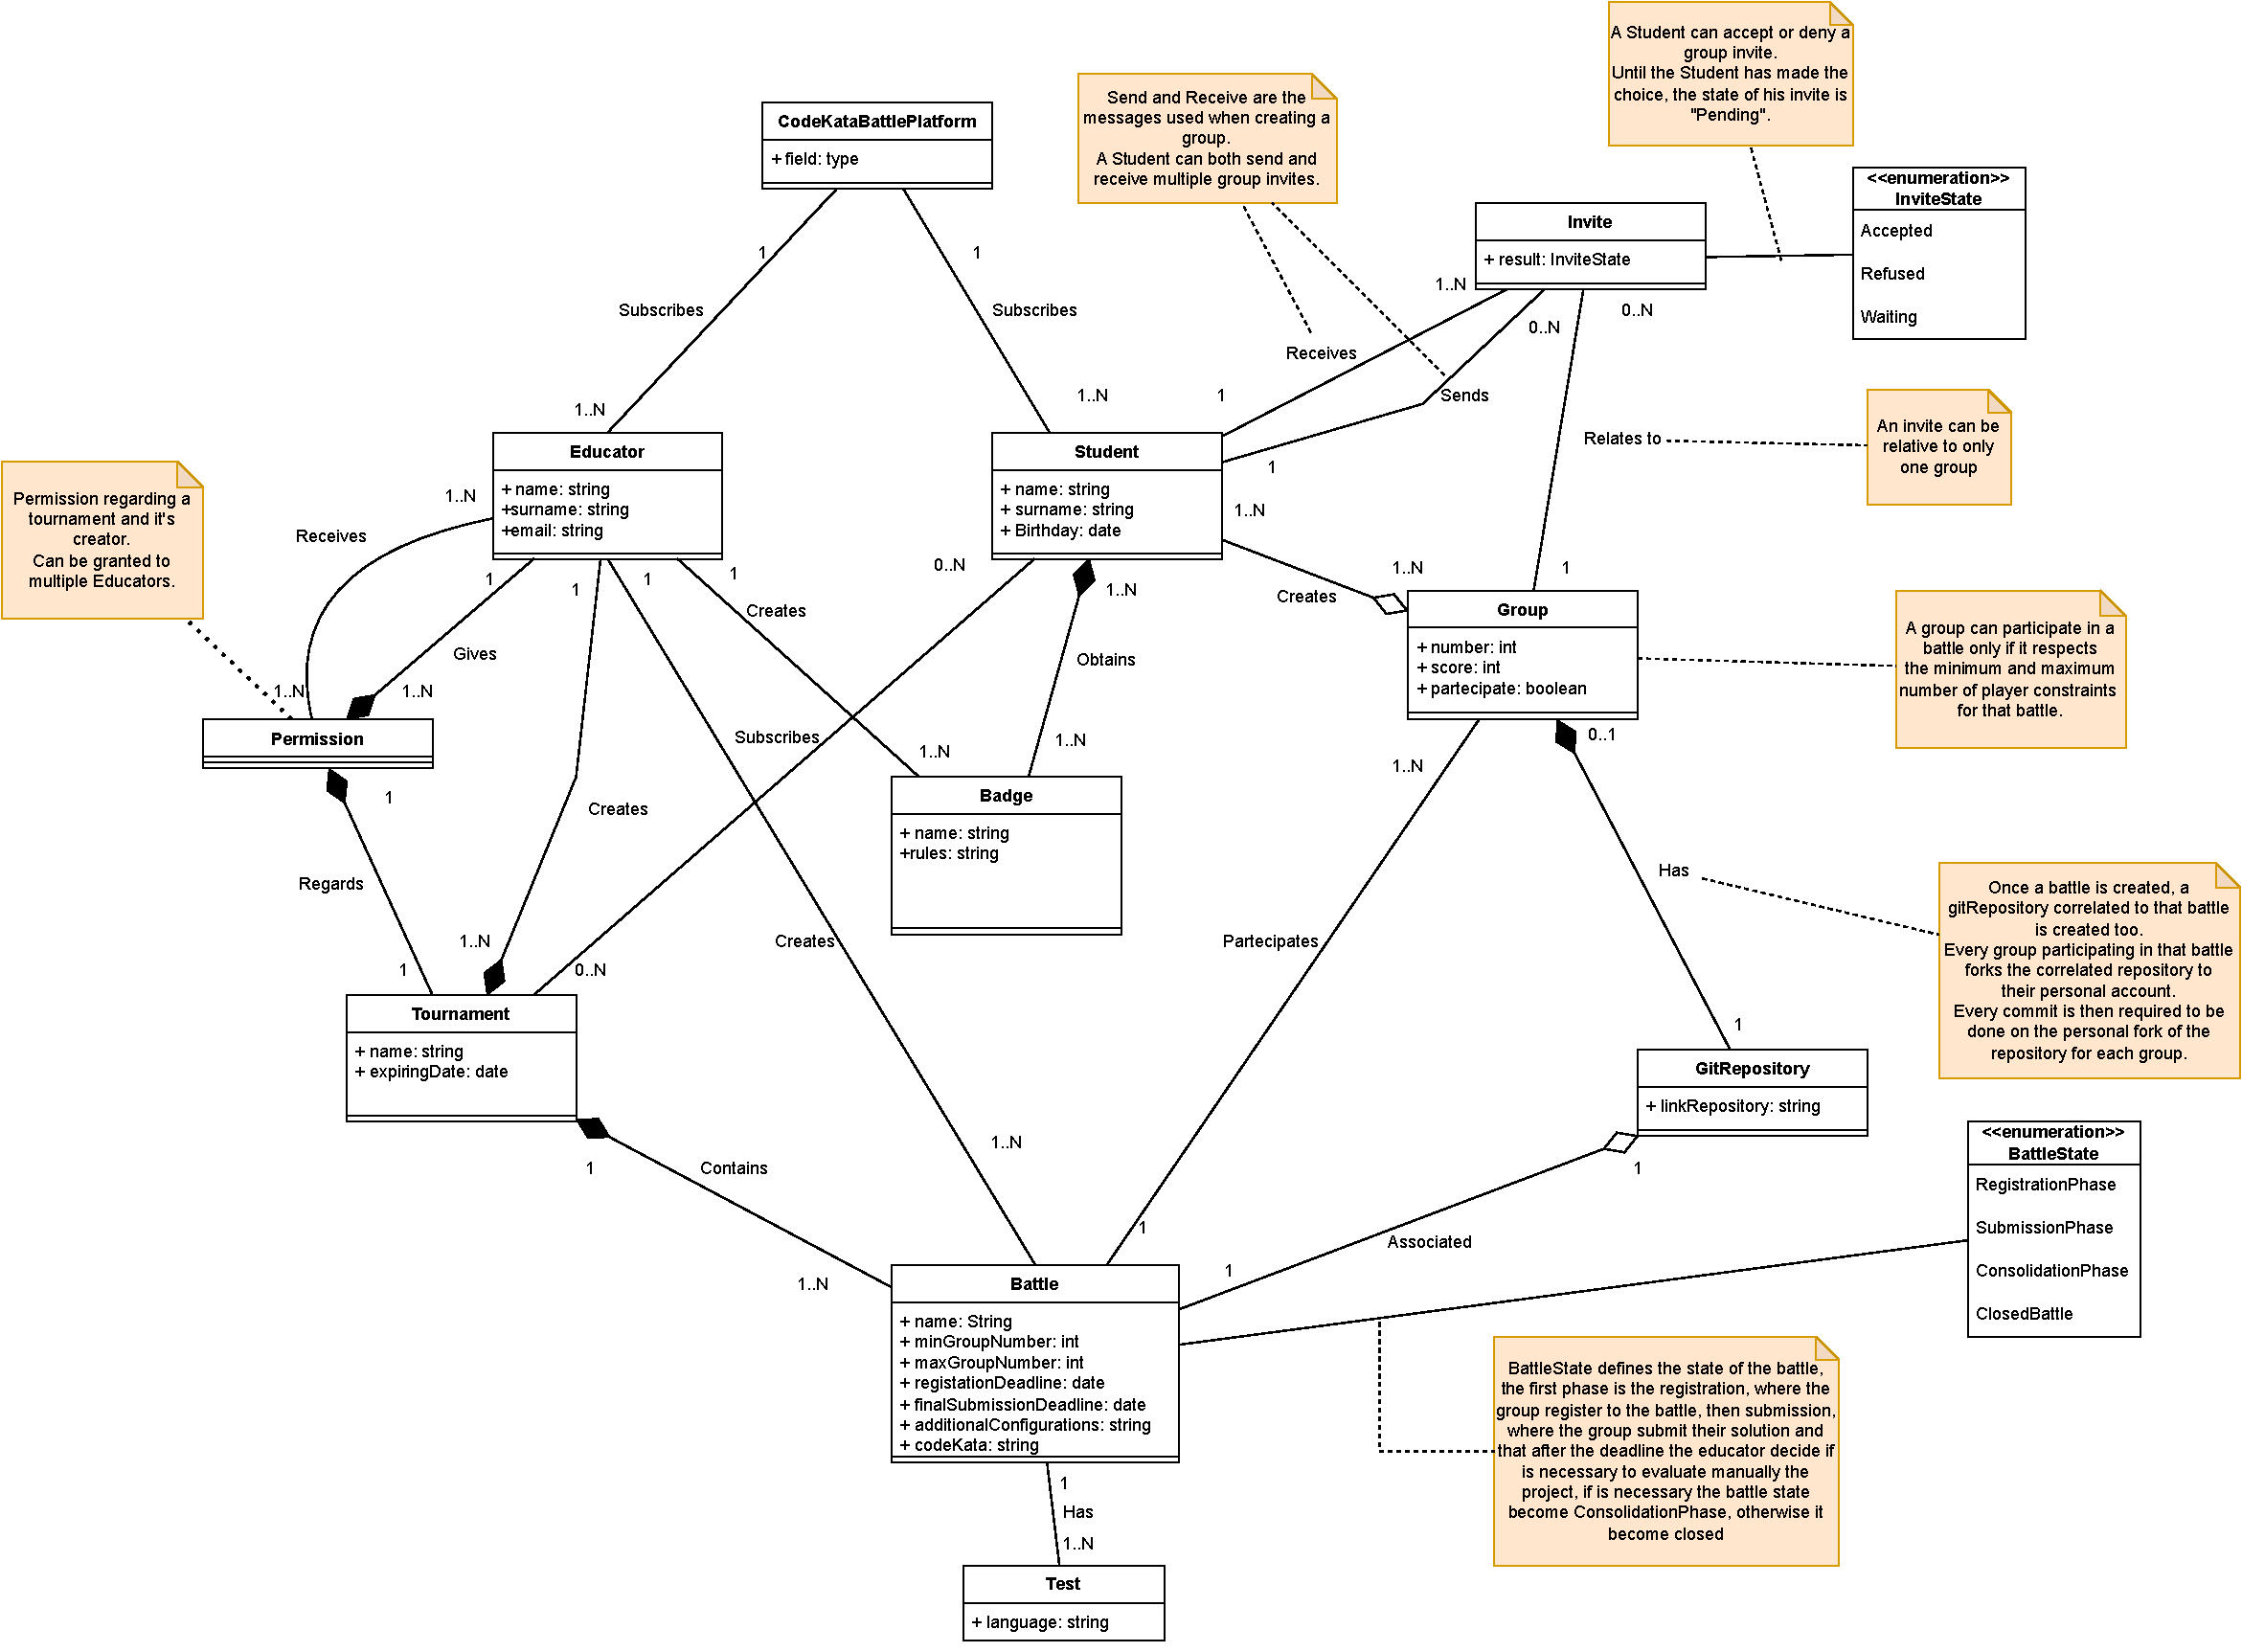
\includegraphics[scale=0.52]{images/ClassDiagram/ClassDiagram.pdf}
    \caption{Class Diagram}
    \label{fig:classDiagram}
\end{figure}

\newpage

\subsection{Product functions}
\subsubsection{Shared functions}
\begin{itemize}
    \item \textbf{Sign-up:} Let the user (Students or Educators) sign-up to the platform.
          \begin{figure}[H]
              \centering
              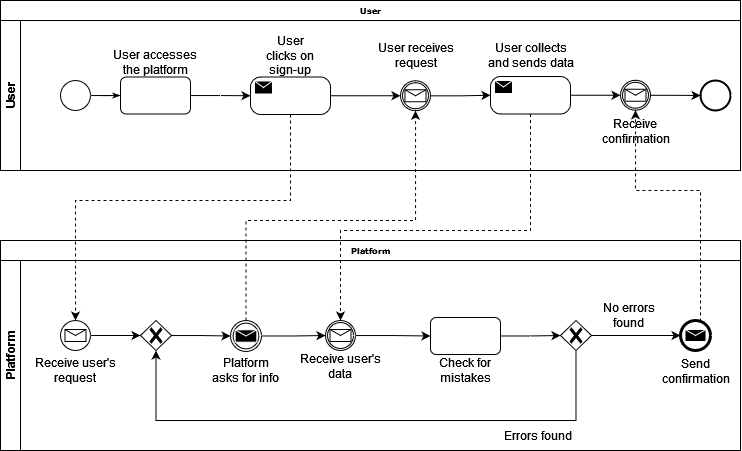
\includegraphics[scale=0.4]{images/BPMN/BPMN1.png}
              \caption{Sign-up BPMN}
              \label{fig:signUpBPMN}
          \end{figure}

    \item \textbf{Visualize student's profile:} Let a user (Student or Educator) visualise the page of a specific Student.
          \begin{figure}[H]
              \centering
              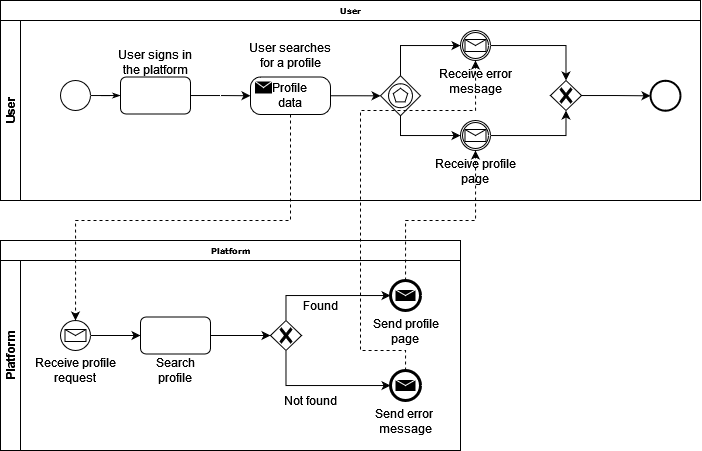
\includegraphics[scale=0.4]{images/BPMN/BPMN2.png}
              \caption{Profile visualization BPMN}
              \label{fig:profileVisualizationBPMN}
          \end{figure}
\end{itemize}

\subsubsection{Student functions}
\begin{itemize}
    \item \textbf{Student subscribes to a tournament:} Let a Student search, according to some parameters 
    (most used programming languages, creation date, number of partecipant, etc...) and subscribe to a tournament, after logging in the platform.
          \begin{figure}[H]
              \centering
              \hspace*{-1.1cm}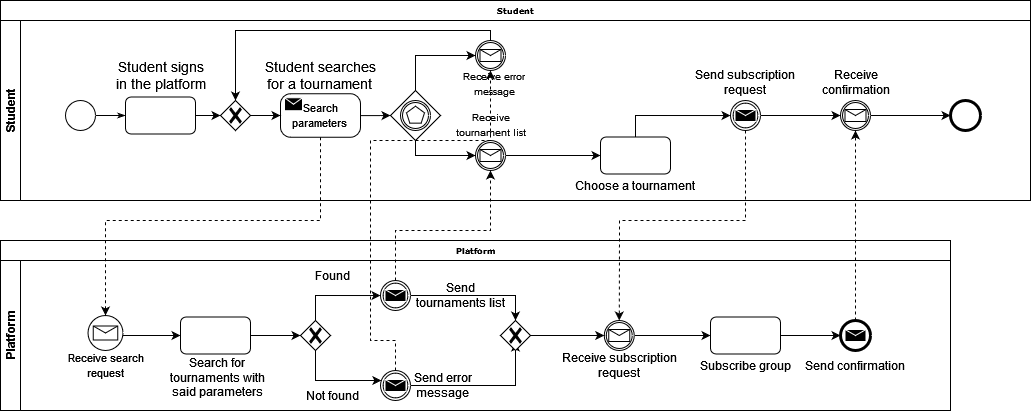
\includegraphics[scale=0.4]{images/BPMN/BPMN3.png}
              \caption{Student's tournament subscription BPMN}
              \label{fig:studTournamentSubBPMN}
          \end{figure}

    \item \textbf{Student join a battle:} Let a student Subscribed to a tournament search for a tournament's battle according 
    to some parameters (programming language requested, expiration date, difficulty, etc...) and join it alone or in a group.
          \begin{figure}[H]
              \centering
              \hspace*{-1.1cm}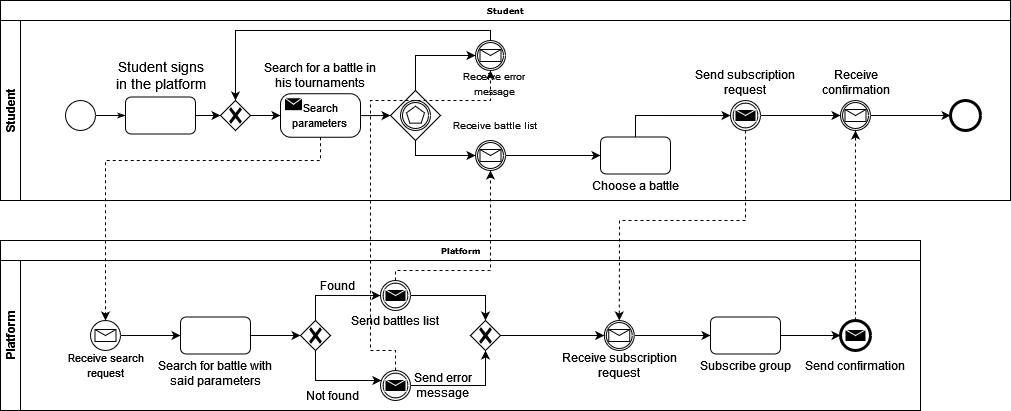
\includegraphics[scale=0.4]{images/BPMN/BPMN4.png}
              \caption{Student's battle joining BPMN}
              \label{fig:studBattleJoinBPMN}
          \end{figure}

          %newpage command used to better format the pdf content
          \newpage

    \item \textbf{Student gets notified of new events:} Notify a Student, if registered to the platform, about new created tournaments and
      new created battles within the tournaments he is subscribed to.
          \begin{figure}[H]
              \centering
              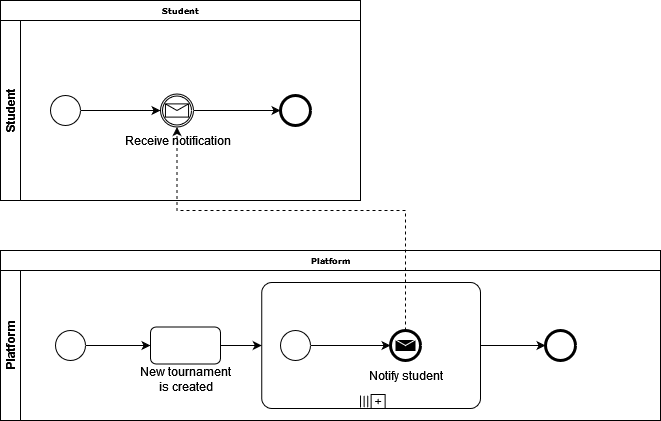
\includegraphics[scale=0.4]{images/BPMN/BPMN5.png}
              \caption{Student notification (Tournament) BPMN}
              \label{fig:studNotificationBPMN}
          \end{figure}

    \item \textbf{Student's solutions get evaluated:} Let a Student, who connects to his forked repository on GitHub, 
    upload his solution and evaluate it according to some parameters.
          \begin{figure}[H]
              \centering
              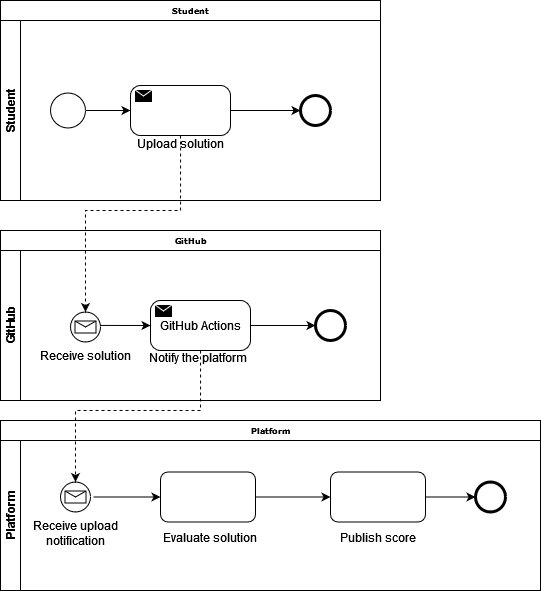
\includegraphics[scale=0.35]{images/BPMN/BPMN6.png}
              \caption{Student's solutions evaluation BPMN}
              \label{fig:studSolEvalBPMN}
          \end{figure}

    \item \textbf{Student form a group for a battle:} Let a Student form a group with other Students in order to face a battle, through invite messages.
          \begin{figure}[H]
              \centering
              \hspace*{-0.9cm}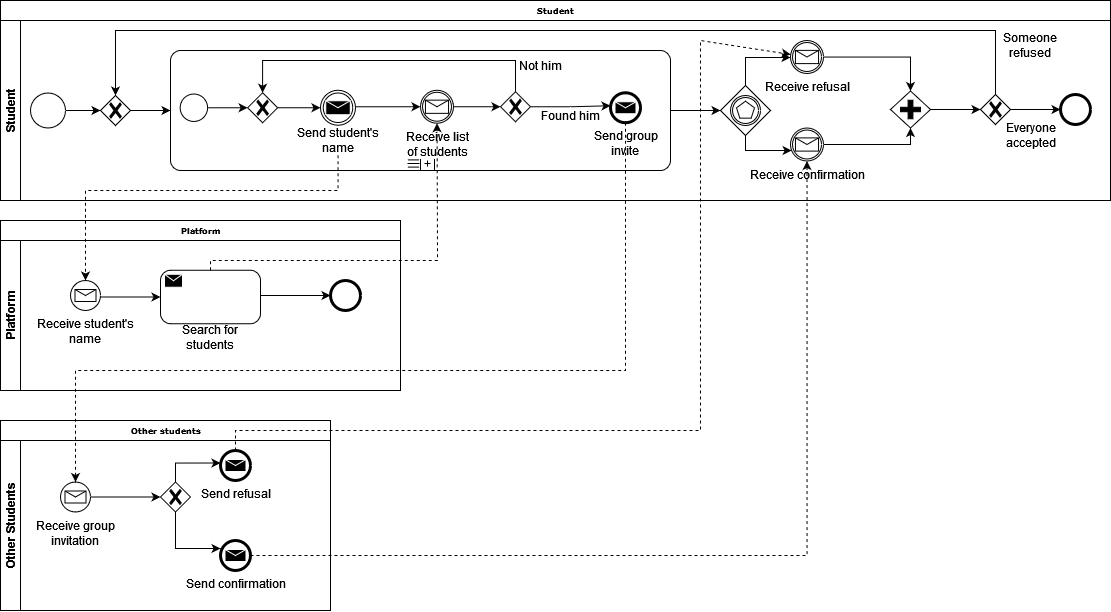
\includegraphics[scale=0.35]{images/BPMN/BPMN7.png}
              \caption{Formation of a group BPMN}
              \label{fig:groupFormationBPMN}
          \end{figure}
\end{itemize}



\subsubsection{Educator functions}
\begin{itemize}
    \item \textbf{Educator create a tournament:} Let an Educator create a new tournament and set its parameters.
          \begin{figure}[H]
              \centering
              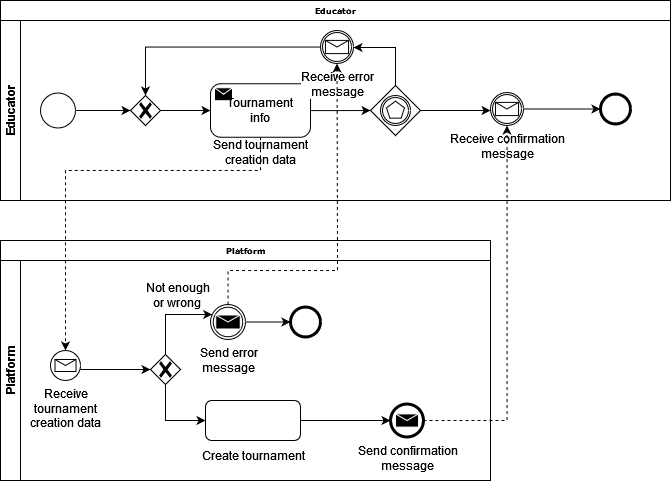
\includegraphics[scale=0.35]{images/BPMN/BPMN8.png}
              \caption{Tournament's creation BPMN}
              \label{fig:TournamentCreationBPMN}
          \end{figure}

    \item \textbf{Educator grant access to a tournament:} Give an Educator the possibility to grant modification access to one of his tournaments to a colleague.
          \begin{figure}[H]
              \centering
              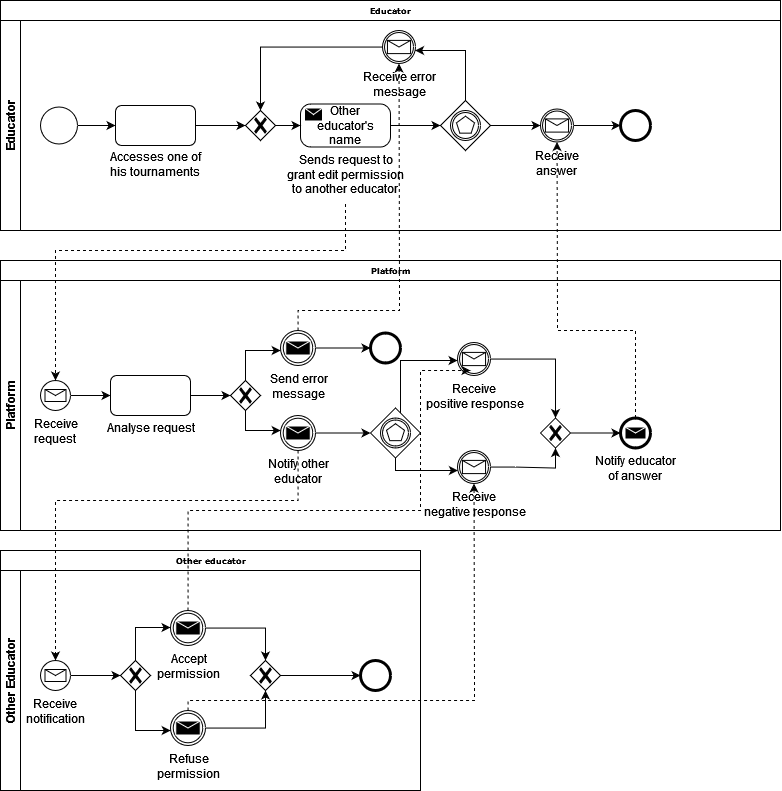
\includegraphics[scale=0.4]{images/BPMN/BPMN10.png}
              \caption{Grant access to tournament BPMN}
              \label{fig:accessGrantTournamentBPMN}
          \end{figure}

          %newpage command used to better format the pdf content
          \newpage

    \item \textbf{Educator close a tournament:} Let an Educator close one of his tournaments.
          \begin{figure}[H]
              \centering
              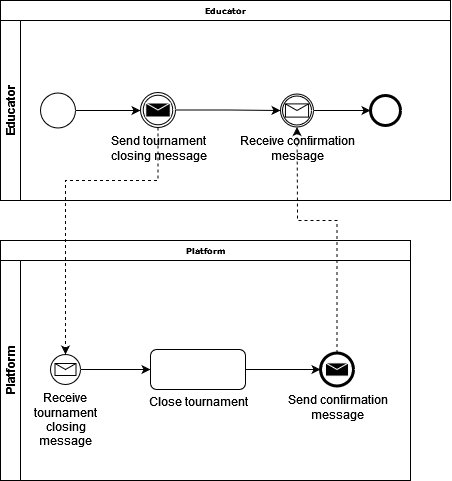
\includegraphics[scale=0.4]{images/BPMN/BPMN9.png}
              \caption{Tournament's closing BPMN}
              \label{fig:TournamentClosingBPMN}
          \end{figure}

    \item \textbf{Educator creates a battle:} Grant an Educator the possibility of creating a battle in tournaments where he has permission to.
          \begin{figure}[H]
              \centering
              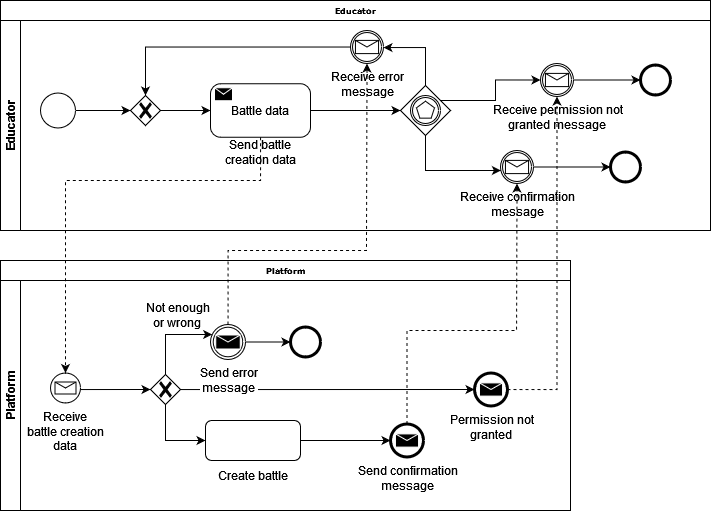
\includegraphics[scale=0.4]{images/BPMN/BPMN11.png}
              \caption{Create battle BPMN}
              \label{fig:createBattleBPMN}
          \end{figure}

    \item \textbf{Educator notified of battle's end:} Educator gets notified about the end of a battle in one of his tournaments, 
    then give him the possibility to manually evaluate the students' solutions.
          \begin{figure}[H]
              \centering
              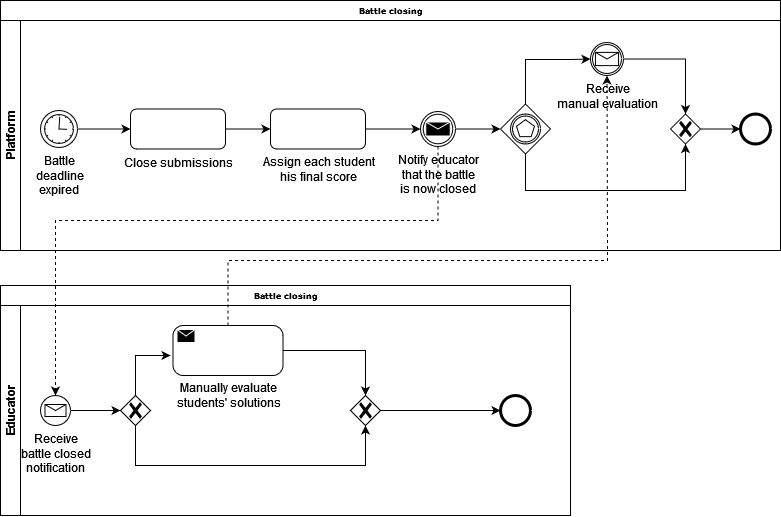
\includegraphics[scale=0.35]{images/BPMN/BPMN12.png}
              \caption{Ending of a battle BPMN}
              \label{fig:battleEndingBPMN}
          \end{figure}
\end{itemize}

\subsection{User characteristics}
CKB platform has 2 different users:
\begin{itemize}
    \item \textbf{Educators:} They are Educators teaching in a school
          environment. They must be qualified to teach. They need to have
          medium to high programming skills, or at least enough knowledge of a programming language
          to create test codes for the battles they want to create.
          Finally they must be provided with an istitutional email in order to properly
          register to the platform.
    \item \textbf{Students:} They are Students of a school that want to
          improve their programming skills. They can be students of any school and they
          can subscribe to tournaments created by an Educators
          employed or not by their school. They must have some knowledge about the GitHub
          platform and how to create GitHub Actions, which are fundamental for the correct
          functioning of the CKB platform.
\end{itemize}

%newpage command used to better format the pdf content
\newpage

\subsection{Assumptions, dependencies and constraints}
\begin{itemize}
    \item[\textbf{D1:}] Students and Educators have access to internet while using the platform.
    \item[\textbf{D2:}] Students and Educators have their own IT device to connect to the application.
    \item[\textbf{D3:}] Students and Educators have to be subscribed to the platform in order to use its features.
    \item[\textbf{D4:}] Students know how to use GitHub actions.
    \item[\textbf{D5:}] Students know how to fork a repository on GitHub.
    \item[\textbf{D6:}] A Student can join a battle only if subscribed to the tournament in which that battle takes place.
    \item[\textbf{D7:}] GitHub platform offers reliable services through its API allowing the CKB platform to always get notified when new code is uploaded by Students.
    \item[\textbf{D8:}] Educator knows how to create new badges and new rules to obtain them.
    \item[\textbf{D9:}] Time information about registration and submission deadlines for tournaments and battles are always correct.
    \item[\textbf{D10:}] Code written by Students cannnot make the platform crash while testing it.
    \item[\textbf{D11:}] Educators upload, when creating a battle, some correct, meaningful and faultproof test cases and automation scripts.
    \item[\textbf{D12:}] Students score is always correctly calculated.
    \item[\textbf{D13:}] Educators can always access to their tournaments and to the ones that has been granted the access to
    by their creators.
    \item[\textbf{D14:}] In order to register to a battle, all the group members must be registered in the tournament
          in which the battle takes place.
    \item[\textbf{D15:}] Students and Educators must have a functioning browser application installed on their devices.
    \item[\textbf{D16:}] Only the Student that created the group can invite other Students in it.
\end{itemize}


\newpage

\pagestyle{SpecificRequirementsStyle}

\section{Specific requirements}
\subsection{External interface requirements}
\subsubsection{User Interfaces}
The system should interface with the users (both Educator and Students) through their
devices, such as: laptops, PC desktops and smartphones, whom must be connected to the internet.
Every user, in order to access the platform, has to connect to an existing domain (like "www.codekatabattle.com"),
by using an appropriate and functioning browser application in order to navigate on the platform.

\subsubsection{Software Interfaces}
The system has to use different software interfaces in order to properly function:
\begin{itemize}
    \item \textbf{DB Interfaces:} The system has to interact with a DB,
          used to store all information necessary for the system to function.
    \item \textbf{GitHub Interfaces:} The system has to interact with the GitHub platform,
          in order to receive the students' solutions. This is done through "GitHub Actions"
          APIs made available by GitHub to automate tasks.
    \item \textbf{Testing Interfaces:} The system needs to test the Students' solutions.
          In order to do this a Testing API must be used.
\end{itemize}

\subsubsection{Hardware Interfaces}
The system has to interface with the hardware components containing
the DB.
\subsubsection{Communication Interfaces}
All communication from and to the CKB platform has to be done through the HTTP/HTTPS protocol.

\newpage
\subsection{Functional requirements}
\subsubsection{Requirements}
\begin{itemize}

    \item[\textbf{R.1}] The CKB platform should allow an unregistered Student to create a new account.
    \item[\textbf{R.2}] The CKB platform should allow an unregistered Educator to create a new account.
    \item[\textbf{R.3}] The CKB platform must allow access to its pages only if the used credentials are correct.
    \item[\textbf{R.4}] The CKB platform must not allow a Student to register more than once in the system.
    \item[\textbf{R.5}] The CKB platform must not allow an Educator to register more than once in the system.
    \item[\textbf{R.6}] Educators can access the platform's services only if they are registered to it.
    \item[\textbf{R.7}] Students can access the platform's services only if they are registered to it.
    \item[\textbf{R.8}] The CKB platform should not allow Students to create tournaments and/or battles.
    \item[\textbf{R.9}] The CKB platform should allow Educators to create battles within a tournament only to the tournament
          creator and to any other Educator that has been granted permission to do so by the tournament creator.
    \item[\textbf{R.10}] The CKB platform must allow Educators to personalise the tournaments they create.
    \item[\textbf{R.11}] The CKB platform must allow Edcuators to personalise the battles they create.
    \item[\textbf{R.12}] The CKB platform must allow Educators to define new obtainable badges for each tournament they
          create.
    \item[\textbf{R.13}] The CKB platform must allow Educators to manually evaluate the solutions uploaded by the Students for the battles that
          the Educators created.
    \item[\textbf{R.14}] The CKB platform must allow Educators to delete or update badges before finalizing a tournament's creation.
    \item[\textbf{R.15}] The CKB platform must allow Educators to define rules to obtain badges in tournaments created by them.
    \item[\textbf{R.16}] The CKB platform must ensure that badges' characteristics respect guidelines regarding their
          name, icon format and rules to obtain them.
    \item[\textbf{R.17}] The CKB platform must allow Educators to create new tournaments.
    \item[\textbf{R.18}] The CKB platform must ensure that tournaments' characteristics respect guidelines regarding their
          name, deadline, access method, programming language.
    \item[\textbf{R.19}] The CKB platform must allow Educators to close tournaments they have created.
    \item[\textbf{R.20}] The CKB platform must ensure that when a tournament is closed, Educators cannot create new battles
          within it.
    \item[\textbf{R.21}] The CKB platform must ensure that if a group uploads a solution to a battle after the submission's deadline,
          that solution will not be considered in the score computation by preventing its upload.
    \item[\textbf{R.22}] The CKB platform must ensure that the score given to a group in a tournament is
          coherent with scores given to the same group in the battles they have partecipated in.
    \item[\textbf{R.23}] The CKB platform must ensure fair competition between group scores. In the tournament's evaluation, the final
          group score should be the average score of all the battles in the tournament for each group. Any battle with no solution submitted will count
          as 0 points.
    \item[\textbf{R.24}] The CKB platform must allow Students to subscribe to a tournament.
    \item[\textbf{R.25}] The CKB platform must allow Students to subscribe to a tournament's battle
          within the registration deadline.
    \item[\textbf{R.26}] The CKB platform must allow Students to submit solutions to a tournament's battle
          within the battle's deadline.
    \item[\textbf{R.27}] The CKB platform must allow Students to send and receive group invitations to and from
          other Students in order to form groups.
    \item[\textbf{R.28}] The CKB platform should allow Students to join a battle only if the group composition rules
          for that battle are complied with.
    \item[\textbf{R.29}] The CKB platform must ensure that solutions uploaded by a Student for a battle are evaluated.
    \item[\textbf{R.30}] The CKB platform must allow a Student to upload solutions to a battle relying on the
          external GitHub service.
    \item[\textbf{R.31}] The CKB platform must ensure that only the latest solution uploaded by a Student for a battle he is subscribed to will
          be taken into consideration for the final score.
    \item[\textbf{R.32}] The CKB platform must allow groups partecipating in a battle to change their solution,
          if the battle's submission deadline hasn't expired yet.
    \item[\textbf{R.33}] The CKB platform must ensure that the score given to a group's solution is
          updated as soon as possible.
    \item[\textbf{R.34}] The CKB platform must allow an Educator to modify the score for a Student's solution.
    \item[\textbf{R.35}] The CKB platform must ensure that when a new tournament is created, all
          Students subscribed to the platform are going to receive a notification.
    \item[\textbf{R.36}] The CKB platform must ensure that when a new battle is created in a tournament,
          all Students subscribed to that tournament are going to receive a notification.
    \item[\textbf{R.37}] The CKB platform must allow Students to visualise the score they obtained in a battle they partecipated in.
    \item[\textbf{R.38}] The CKB platform must allow Students to visualise the score they obtained in a tournament they partecipated in.
    \item[\textbf{R.39}] The CKB platform must allow Students to visualise the badges they obtained.
    \item[\textbf{R.40}] The CKB platform must ensures that battles' characteristics respect guidelines
          regarding their name, deadlines, programming language, number of member per group.
\end{itemize}

%newpage command used to better format the pdf content
\newpage

\subsubsection{Use case diagrams}
\begin{itemize}
    \item \underline{\large{\textbf{Student}}}
          \begin{figure}[H]
              \centering
              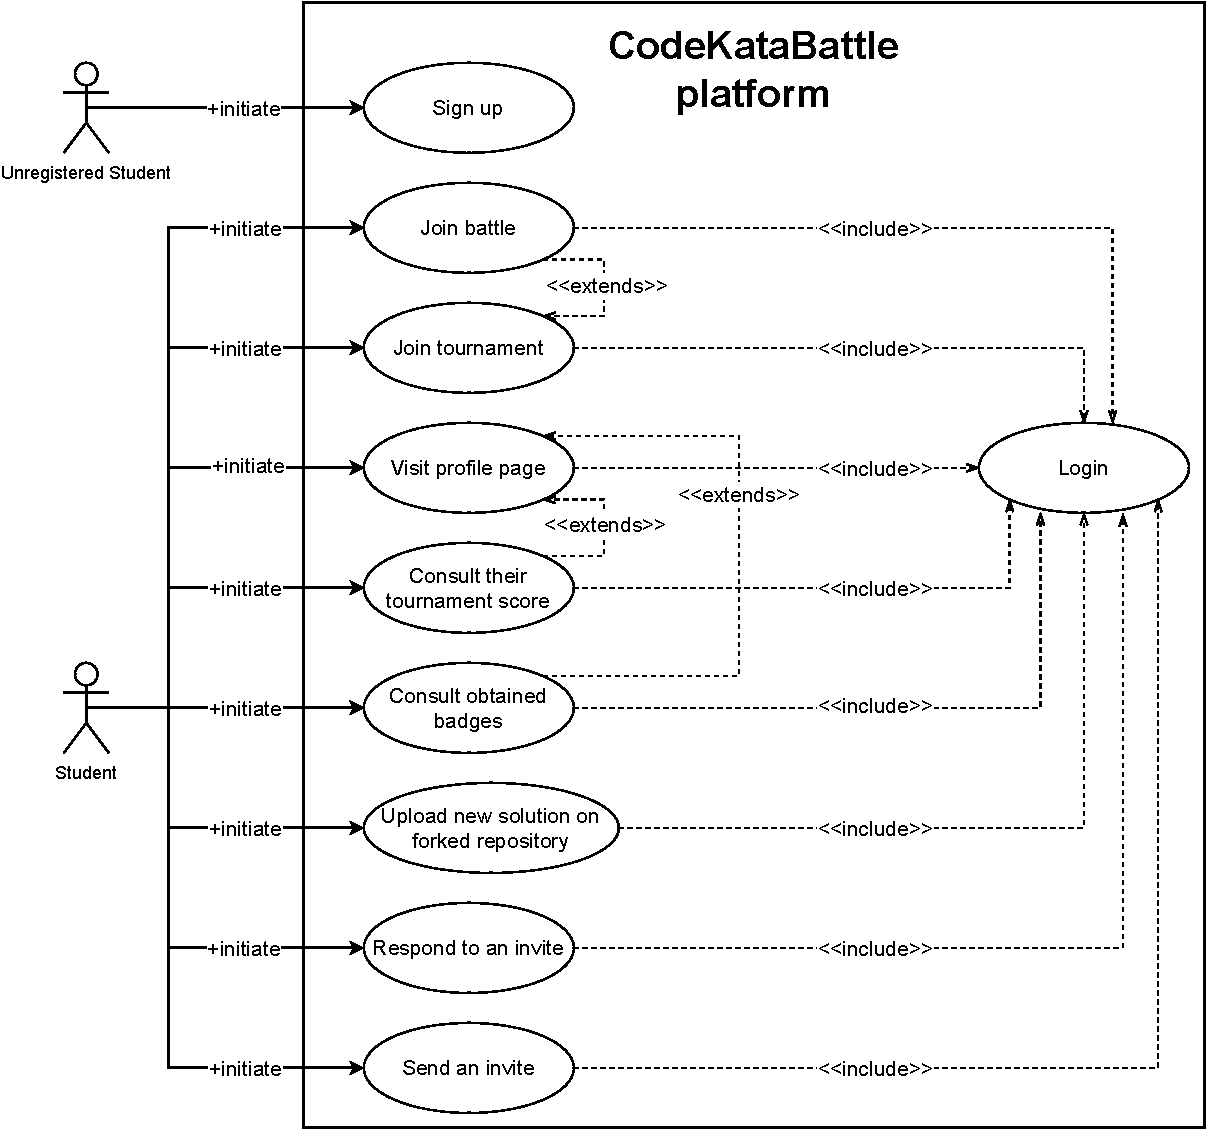
\includegraphics[scale=0.55]{images/3.2.2_UseCaseDiagrams/CaseDiagramStudent.pdf}
              \caption{Student use case diagram}
              \label{fig:studentUseCaseDiagram}
          \end{figure}

          N.B: The repository citated in this diagram, on which the student upload their solution, it is not
          part of the platform. The system, in fact, relies on a third party service (GitHub) to handle the repository.
          This use case was specified in order to better clarify the tight interaction between the system and the Student through the GitHub service.

          %newpage command used to better format the pdf content
          \newpage

    \item \underline{\large{\textbf{Educator}}}
          \begin{figure}[H]
              \centering
              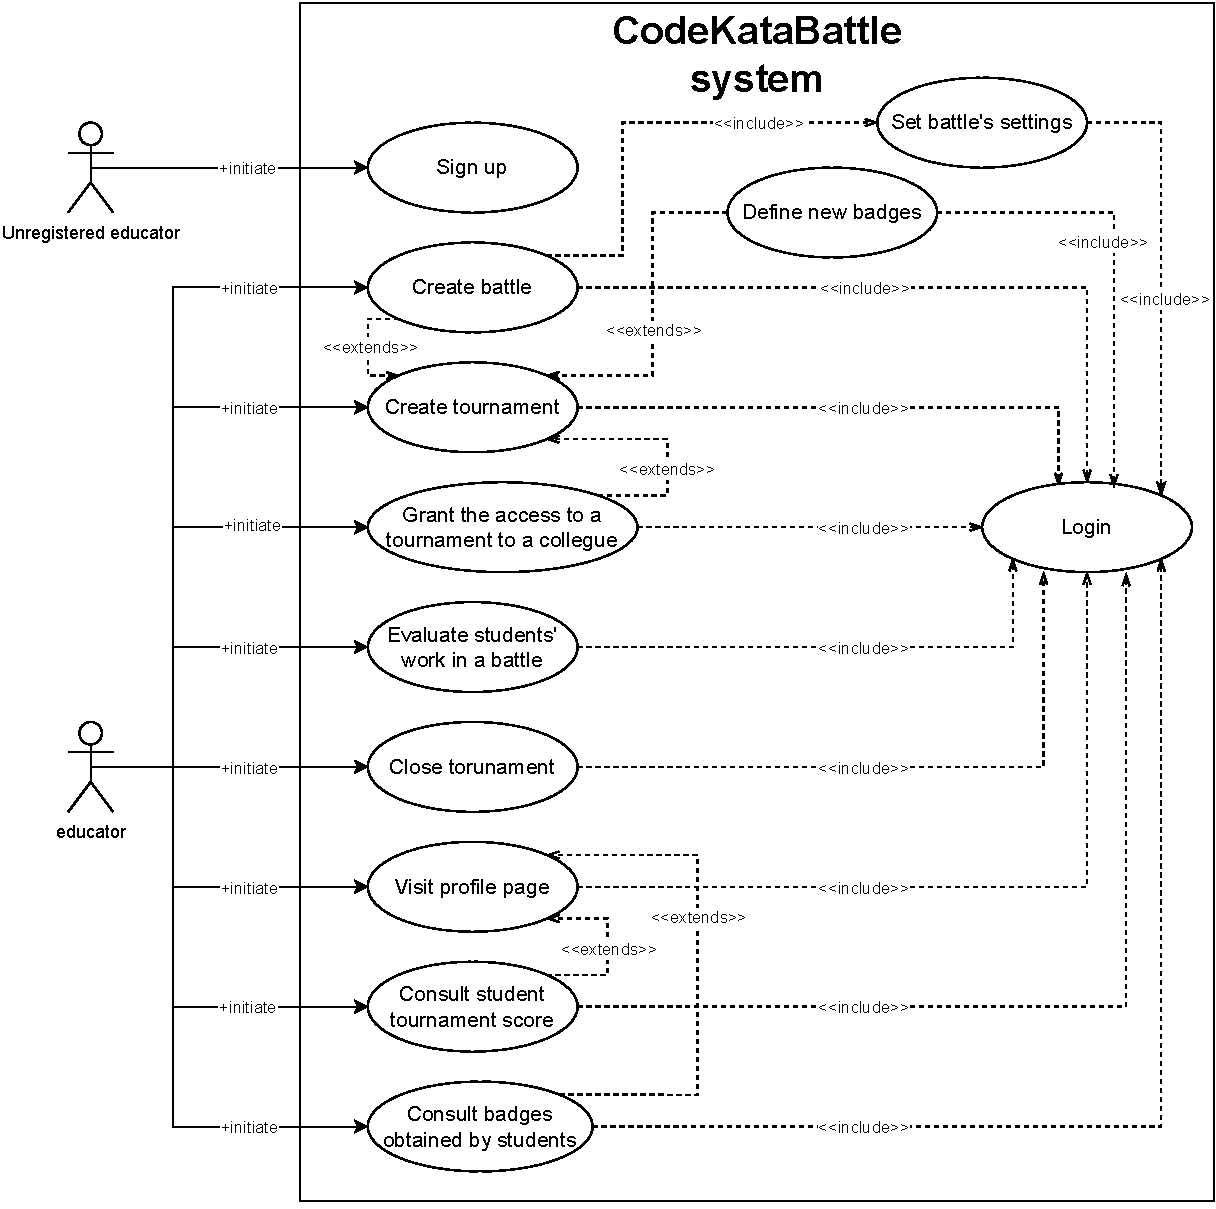
\includegraphics[scale=0.55]{images/3.2.2_UseCaseDiagrams/CaseDiagramEducator.pdf}
              \caption{Educator use case diagram}
              \label{fig:educatorUseCaseDiagram}
          \end{figure}
    \item \underline{\large{\textbf{GitHub}}}
          \begin{figure}[H]
              \centering
              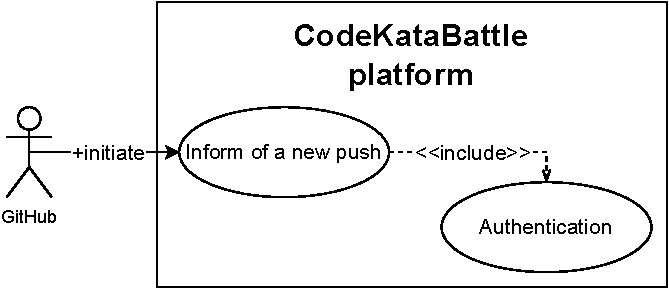
\includegraphics[scale=0.55]{images/3.2.2_UseCaseDiagrams/CaseDiagramGitHub.pdf}
              \caption{GitHub use case diagram}
              \label{fig:gitHubUseCaseDiagram}
          \end{figure}

\end{itemize}
\subsubsection{Use cases w/ sequence diagrams}
\begin{enumerate}
    \item[\textbf{1.}] \textbf{Student sign-up to the platform}

          \begin{xltabular}{\textwidth}
              {| >{\raggedright\arraybackslash}g | >{\raggedright\arraybackslash}X |}
              \hline
              \endfirsthead
              \hline
              \endhead
              \endfoot
              \hline
              \endlastfoot




              \textbf{Name} & Student sign-up \\
              \hline
              \textbf{ID} & UC.1 \\
              \hline
              \textbf{Actors} & Unregistered Student \\
              \hline
              \textbf{Entry condition} & Student wants to register to the platform \\
              \hline
              \textbf{Flow of events} &    \begin{enumerate}
                  \item[1.] Student opens CKB platform.
                  \item[2.] Student presses the sign-up button.
                  \item[3.] Student fills the form with all the required informations (name, surname, username
                        attended school, email, password, ...), accepts the "Terms \& Conditions".
                  \item[4.] Student clicks on a "Confirm" button to confirm.
                  \item[5.] CKB platform validates the personal information inserted by the Student.
                  \item[6.] CBK platform displays a confirmation message.
                  \item[7.] CKB platform sends an email notification to the Student regarding the registration outcome.
              \end{enumerate}   \\
              \hline
              \textbf{Exit condition} & Student's account is created, and its data are saved into the system.\\
              \hline
              \textbf{Exceptions} &     \begin{itemize}
                  \item[4.1] Email already used to register another account, or inexisting.
                  \item[4.2] Inserted attended school non existings.
                  \item[4.3] Username contains forbidden characters.
                  \item[4.4] Password doesn't respect security standards.
                        \begin{itemize}
                            \item[$\rightarrow$] Unregistered Student gets notified of the registration failure through an
                                  error message and flow restarts from point 3.
                        \end{itemize}
              \end{itemize}

          \end{xltabular}


          \begin{figure}[H]
              \centering
              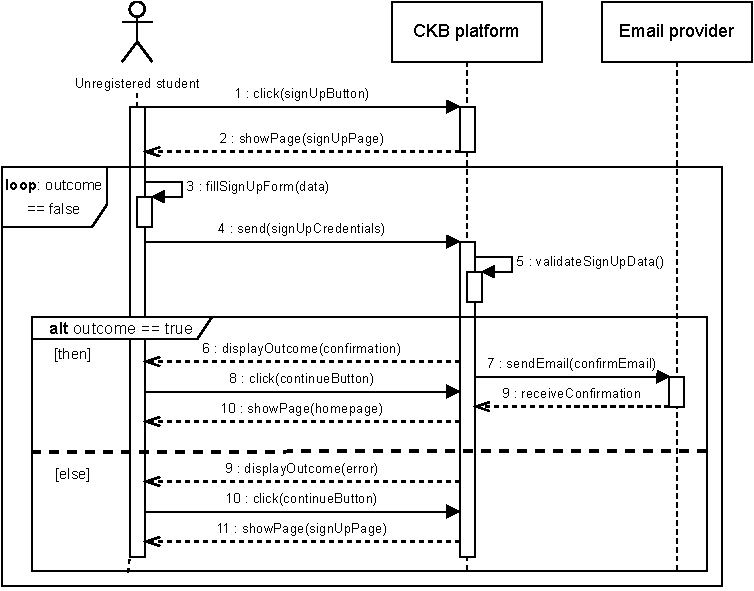
\includegraphics[scale=0.95]{SequenceDiagrams/StudentSignUpSeqDiagram.pdf}
              \caption{Student sign-up sequence diagram}
              \label{fig:StudentSignUpSeqDiagram}
          \end{figure}

    \newpage
    \item[\textbf{2.}] \textbf{Educator sign-up to the platform}
          \begin{xltabular}{\textwidth}
              {| >{\raggedright\arraybackslash}g | >{\raggedright\arraybackslash}X |}
              \hline
              \endfirsthead
              \hline
              \endhead
              \endfoot
              \hline
              \endlastfoot




              \textbf{Name} & Educator sign-up \\
              \hline
              \textbf{ID} & UC.2 \\
              \hline
              \textbf{Actors} & Unregistered Educator \\
              \hline
              \textbf{Entry condition} & Educator wants to register to the platform \\
              \hline
              \textbf{Flow of events} &    \begin{enumerate}
                  \item[1.] Educator opens CKB platform.
                  \item[2.] Educator presses the sign-up button.
                  \item[3.] Educator fills the form with all the required informations (name, surname, username
                        school in which teaches, istitutional email, password, ...), accepts the "Terms \& Conditions".
                  \item[4.] Educator clicks on a "Confirm" button to confirm.
                  \item[5.] CKB platform validates the personal information inserted by the Educator.
                  \item[6.] CBK platform displays a confirmation message.
                  \item[7.] CKB platform sends an email notification to the Educator regarding the registration outcome.
              \end{enumerate} \\
              \hline
              \textbf{Exit condition} & Educator's account is created, and its data are saved into the system. \\
              \hline
              \textbf{Exceptions} &     \begin{itemize}
                  \item[4.1] Email already used to register another account, or inexisting.
                  \item[4.2] Inserted school's details non correct.
                  \item[4.3] Username contains forbidden characters.
                  \item[4.4] Password don't respect security standards.
                        \begin{itemize}
                            \item[$\rightarrow$] Unregistered Educator gets notified of the registration failure through an error message
                                  and flow restart from point 3.
                        \end{itemize}
              \end{itemize}
          \end{xltabular}

          \begin{figure}[H]
              \centering
              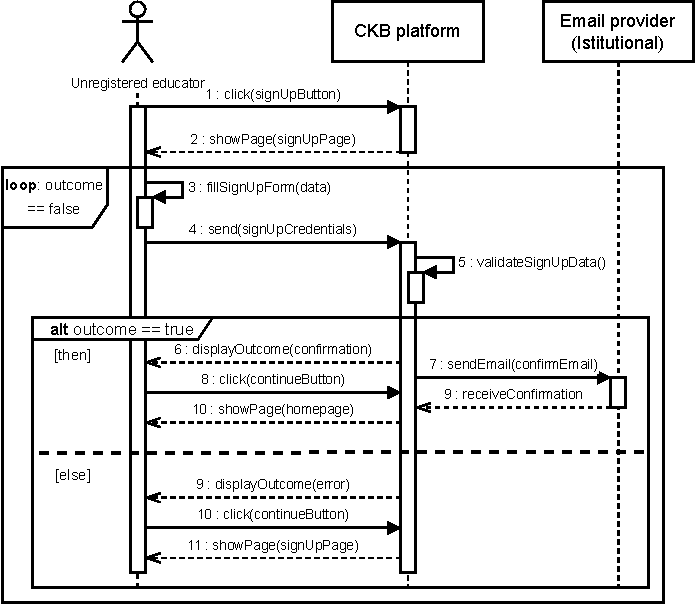
\includegraphics[scale=0.95]{SequenceDiagrams/Sequence2.pdf}
              \caption{Educator sign-up sequence diagram}
              \label{fig:EducatorSignUpSeqDiagram}
          \end{figure}

    \item[\textbf{3.}] \textbf{Educator creates a new tournament}
          \begin{xltabular}{\textwidth}
              {| >{\raggedright\arraybackslash}g | >{\raggedright\arraybackslash}X |}
              \hline
              \endfirsthead
              \hline
              \endhead
              \endfoot
              \hline
              \endlastfoot




              \textbf{Name} & Tournament creation\\
              \hline
              \textbf{ID} & UC.3\\
              \hline
              \textbf{Actors} & Educator, Student\\
              \hline
              \textbf{Entry condition} & Educator has logged in the platform and
              wants to create a new tournament\\
              \hline
              \textbf{Flow of events} &    \begin{enumerate}
                  \item[1.] Educator clicks on a "Create tournament" button.
                  \item[2.] Educator fills a form on the page that has appeared with tournament details,
                        such as: deadline, allowed programming languages, name, access method, etc.
                  \item[3.] Eventually the Educator defines new badges for the tournament (see UC.4)
                  \item[4.] Educator clicks on a "Confirmation" button.
                  \item[5.] CKB platform checks the validity of the informations inserted by the Educator.
                  \item[6.] CKB platform displays a message that confirms that the tournament
                        has been created successfully.
              \end{enumerate} \\
              \hline
              \textbf{Exit condition} & Tournament is created by saving its data into the system
              and the platform sends a notification to all the Students registered to the platform about the new tournament created.
              Educator is led back to the riepilogative page of the tournament creation. \\
              \hline
              \textbf{Exceptions} &    \begin{itemize}
                  \item[5.1] Tournament's name contain forbidden characters.
                  \item[5.2] Deadline inserted for the tournament is invalid.
                  \item[5.3] Tournament's access method has been configured wrongly.
                  \item[5.4] The programming language inserted is not recognized by the platform.
                        \begin{itemize}
                            \item[$\rightarrow$] Educator gets notified about the tournament's creation failure
                                  through an error message displayed by the platform. The flow restarts from point 2.
                        \end{itemize}
              \end{itemize}
          \end{xltabular}

          \begin{figure}[H]
              \centering
              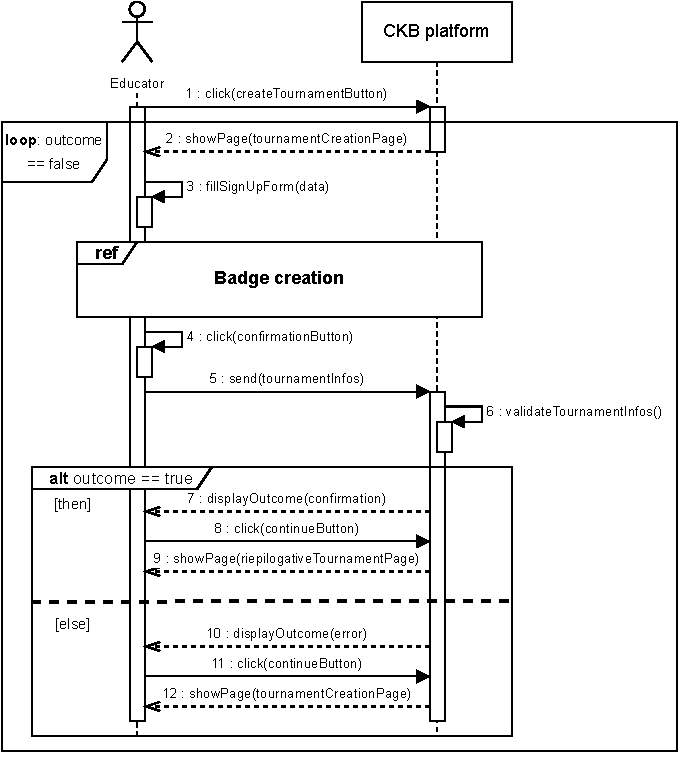
\includegraphics[scale=0.95]{SequenceDiagrams/Sequence3.pdf}
              \caption{Educator creates a new tournament sequence diagram}
              \label{fig:TournamentCreationSeqDiagram}
          \end{figure}

    \newpage
    \item[\textbf{4.}] \textbf{Educator creates new badges}
          \begin{xltabular}{\textwidth}
              {| >{\raggedright\arraybackslash}g | >{\raggedright\arraybackslash}X |}
              \hline
              \endfirsthead
              \hline
              \endhead
              \endfoot
              \hline
              \endlastfoot




              \textbf{Name} & Badges creation\\
              \hline
              \textbf{ID} & UC.4\\
              \hline
              \textbf{Actors} & Educator\\
              \hline
              \textbf{Entry condition} & Educator has logged in the platform, he's creating a new tournament and wants to
              define new badges for that tournament\\
              \hline
              \textbf{Flow of events} &    \begin{enumerate}
                  \item[1.] Educator clicks on the "Create badge" button on the tournament
                        creation page.
                  \item[2.] On the new page that appeared, the Educator defines badge's
                        characteristics, such as: name, value, icon, rules to obtain it, ...
                  \item[3.] Educator clicks on "Confirm" button in order to confirm its choices.
                  \item[4.] CKB platform checks if all the badge informations are well defined.
                  \item[5.] CKB platform displays a message that confirms the successfull creation
                        of a new badge, and that the badge has been added to the tournament.
              \end{enumerate} \\
              \hline
              \textbf{Exit condition} & Badge is created, its data are saved and associated to the
              tournament for which is being created by the Educator. The Educator is then led back to the
              tournament creation page. \\
              \hline
              \textbf{Exceptions} &    \begin{itemize}
                  \item[4.1] Badge's name contain forbidden characters
                  \item[4.2] The image uploaded as icon is too big or has an unsupported format.
                  \item[4.3] Badge's rules are not well defined.
                  \item[4.4] Some badge's features have been left empty
                        \begin{itemize}
                            \item[$\rightarrow$] Educator gets notified about the badge's creation process failure
                                   through an error message displayed by the platform. Flow restarts from point 2.
                        \end{itemize}
              \end{itemize}
          \end{xltabular}

          \begin{figure}[H]
              \centering
              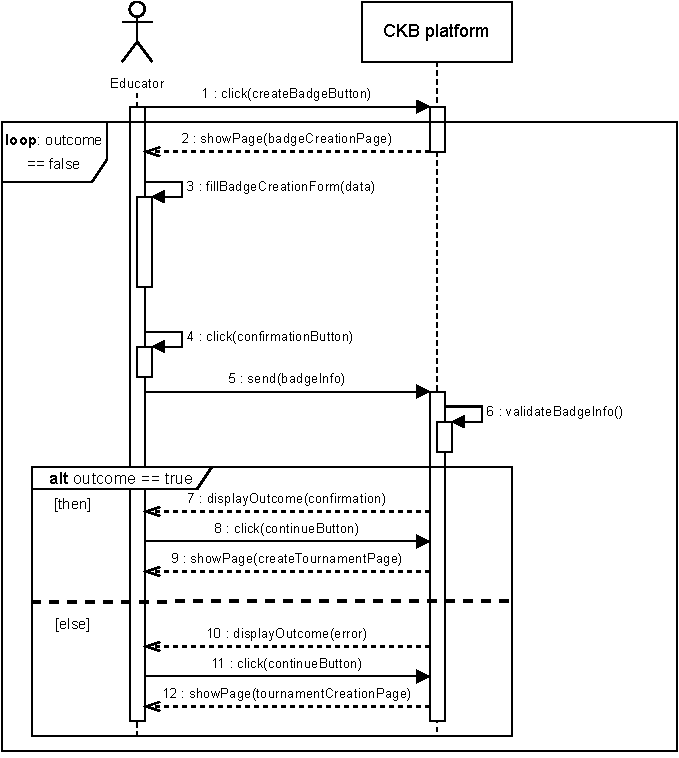
\includegraphics[scale=0.875]{SequenceDiagrams/Sequence4.pdf}
              \caption{Educator creates new badges for a tournament sequence diagram}
              \label{fig:BadgesCreationSeqDiagram}
          \end{figure}

    \item[\textbf{5.}] \textbf{Educator deletes a badge}
          \begin{xltabular}{\textwidth}
              {| >{\raggedright\arraybackslash}g | >{\raggedright\arraybackslash}X |}
              \hline
              \endfirsthead
              \hline
              \endhead
              \endfoot
              \hline
              \endlastfoot




              \textbf{Name} & Deletion \& update of a badge\\
              \hline
              \textbf{ID} & UC.5\\
              \hline
              \textbf{Actors} & Educator\\
              \hline
              \textbf{Entry condition} & Educator has logged in the platform, has started the creation of a new
              tournament in which he has already created at least one badge and wants to delete and/or update one of this tournament's badges.\\
              \hline
              \textbf{Flow of events} &    \begin{enumerate}
                  \item[1.] Educator clicks on the update button related to the badge and
                        present on the tournament creation page.
                  \item[2.] CKB platform shows a modifiable form, filled with the
                        badge's data that the Educator wants to modify.
                  \item[3.] Educator proceeds to modify the badge's data.
                  \item[4.] CKB platform tries to validate the new data.
                  \item[5.] Update is confirmed with the display of a confirmation message by the CKB platform.
                  \item[6.] Educator clicks on the delete button related to
                        the badge and present on the tournament creation page.
                  \item[7.] CKB platform show a message requiring confirmation
                        for the badge deletion.
                  \item[8.] Educator presses the confirmation button.
                  \item[9.] CKB platform deletes the badge and forwards the Educator
                        back to the previous page.
              \end{enumerate} \\
              \hline
              \textbf{Exit condition} & Deleted badges are removed from the tournament and their data is removed
              from the platform. The modifications of the updated badges are committed to the platform. The Educator
              is led back to the tournament creation page. \\
              \hline
              \textbf{Exceptions} &    \begin{itemize}
                  \item[4.1] Badge's updated name contain forbidden characters.
                  \item[4.2] The new image uploaded as icon is too big or has an unsupported format.
                  \item[4.3] New badge's rules are not well defined.
                  \item[4.4] Some badge's features have been left empty.
                        \begin{itemize}
                            \item[$\rightarrow$] Badge is not updated, Educator is led back to
                                  the tournament creation page. (point 1.).
                        \end{itemize}
                  \item[6.1] Educator presses the cancel button
                        \begin{itemize}
                            \item[$\rightarrow$] Delete procedure is stopped, Educator
                                  is led back to the tournament creation page (point 6.).
                        \end{itemize}

              \end{itemize}
          \end{xltabular}

          \begin{figure}[H]
              \centering
              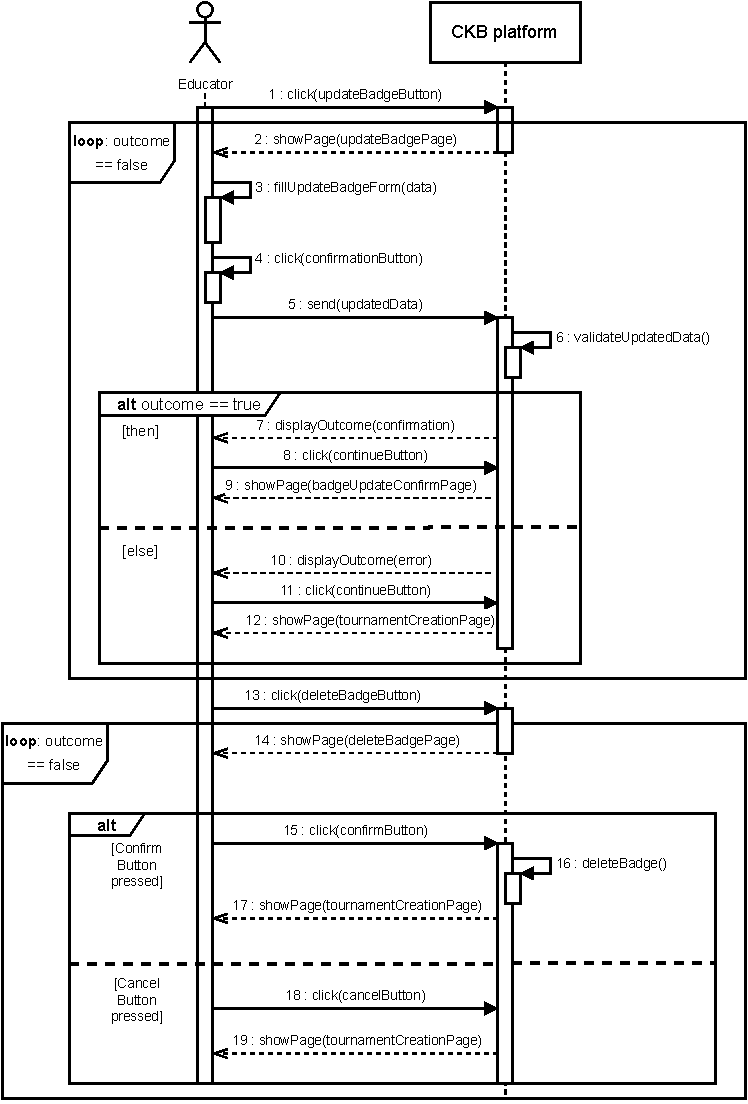
\includegraphics[scale=0.95]{SequenceDiagrams/Sequence5.pdf}
              \caption{Educator deletes and/or updates a tournament's badge(s) sequence diagram}
              \label{fig:DeletionUpdateBadgesSeqDiagram}
          \end{figure}

    \item[\textbf{6.}] \textbf{Educator creates a new battle}
          \begin{xltabular}{\textwidth}
              {| >{\raggedright\arraybackslash}g | >{\raggedright\arraybackslash}X |}
              \hline
              \endfirsthead
              \hline
              \endhead
              \endfoot
              \hline
              \endlastfoot




              \textbf{Name} & Battle creation\\
              \hline
              \textbf{ID} & UC.6\\
              \hline
              \textbf{Actors} & Educator\\
              \hline
              \textbf{Entry condition} & Educator has logged in the platform, has created at least one tournament
              and wants to add a battle in a specific tournament. \\
              \hline
              \textbf{Flow of events} &    \begin{enumerate}
                  \item[1.] Educator opens the page related to a specific tournament
                        which he has created.
                  \item[2.] Educator clicks on the button used to create a new battle.
                  \item[3.] Educator fills the form shown by the platform with informations
                        related to the battle that he wants to create (name, programming languages
                        allowed, maximum and minimum number of students for each partecipating
                        group, registration and submission deadlines, ...).
                  \item[4.] Educator clicks on a button to confirm.
                  \item[5.] CKB platform validates the battle characteristics.
                  \item[6.] CKB platform displays a confirmation message of the successfull
                        battle's creation.
              \end{enumerate} \\
              \hline
              \textbf{Exit condition} & New battle, with characteristics specified by the Educator,
              is created within the tournament chosen by the Educator himself. All the Students subscribed to the tournament
              in which the battle has been created get notified. Educator is then led to the riepilogative
              page of the tournament's battles.
              \\
              \hline
              \textbf{Exceptions} &    \begin{itemize}
                  \item[3.1] Battle's name contains forbidden characters.
                  \item[3.2] A programming language inserted is not included in the tournament
                        allowed programming languages.
                  \item[3.3] The specified number of minimum or maximum Students for each group
                        is beyond upper and/or lower limits imposed by the platform.
                  \item[3.4] Registration deadline inserted for the battle is not valid or
                        bigger than the submission one.
                  \item[3.5] Submission deadline inserted for the battle is not valid or
                        smaller than the registration one.
                        \begin{itemize}
                            \item[$\rightarrow$] Educator gets notified about battle's creation failure
                                  by the platform through an error message. The flow restarts from point 3.
                        \end{itemize}
              \end{itemize}
          \end{xltabular}

          \begin{figure}[H]
              \centering
              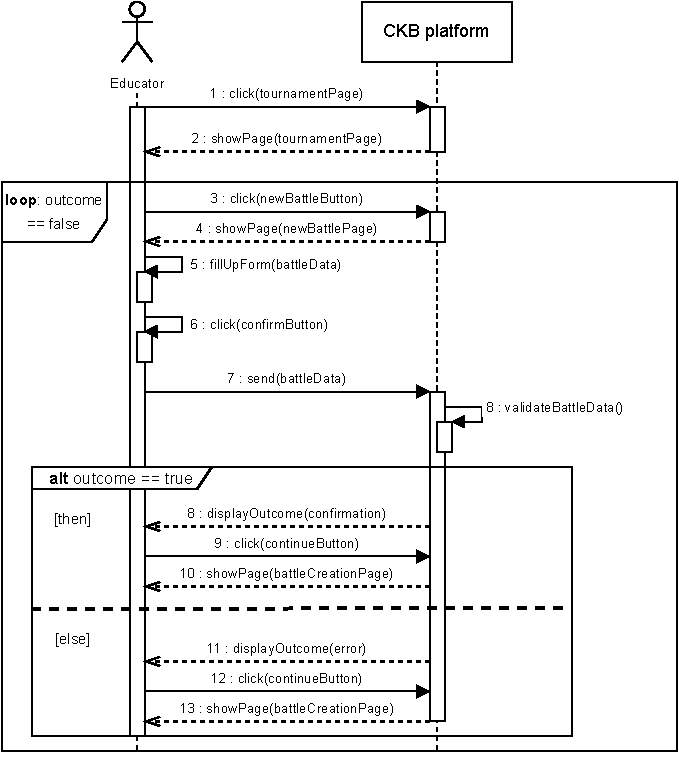
\includegraphics[scale=0.95]{SequenceDiagrams/Sequence6.pdf}
              \caption{Educator creates a new battle sequence diagram}
              \label{fig:BattleCreationSeqDiagram}
          \end{figure}

    \newpage
    \item[\textbf{7.}] \textbf{Educator closes a tournament}
          \begin{xltabular}{\textwidth}
              {| >{\raggedright\arraybackslash}g | >{\raggedright\arraybackslash}X |}
              \hline
              \endfirsthead
              \hline
              \endhead
              \endfoot
              \hline
              \endlastfoot




              \textbf{Name} & Tournament closure\\
              \hline
              \textbf{ID} & UC.7\\
              \hline
              \textbf{Actors} & Educator\\
              \hline
              \textbf{Entry condition} & Educator has logged in the platform, has created at least one tournament
              and wants to close one of them in order to end the competition \\
              \hline
              \textbf{Flow of events} &    \begin{enumerate}
                  \item[1.] Educator accesses the tournament's page
                        that he wants to close.
                  \item[2.] Educator checks whether there are battles that
                        aren't already closed.
                  \item[3.] Educator clicks on the tournament's close button,
                        then clicks on the confirm button.
                  \item[4.] CKB platform verifies if there are no battles
                        still active within the tournament.
                  \item[5.] CKB platform notifies the Educator through
                        a message that confirms the deletion of the tournament.
              \end{enumerate} \\
              \hline
              \textbf{Exit condition} & The chosen tournament is closed, its data are kept saved in
              order to create an history of tournaments. Educator is led back to the riepilogative
              page of the tournaments he created. \\
              \hline
              \textbf{Exceptions} &    \begin{itemize}
                  \item[2.1] Active battles are found within the tournament.
                        \begin{itemize}
                            \item[$\rightarrow$] Educator can prevent 
                                  other Educators from creating new battles if he's the tournament
                                  creator. The flow restarts from point 1.
                        \end{itemize}
                  \item[4.1] Active battles are found within the tournament.
                        \begin{itemize}
                            \item[$\rightarrow$] CKB platform interrupts the tournament
                                  deletion and displays an error message to the Educator. Flow
                                  restarts from point 1.
                        \end{itemize}
              \end{itemize}
          \end{xltabular}

          \begin{figure}[H]
              \centering
              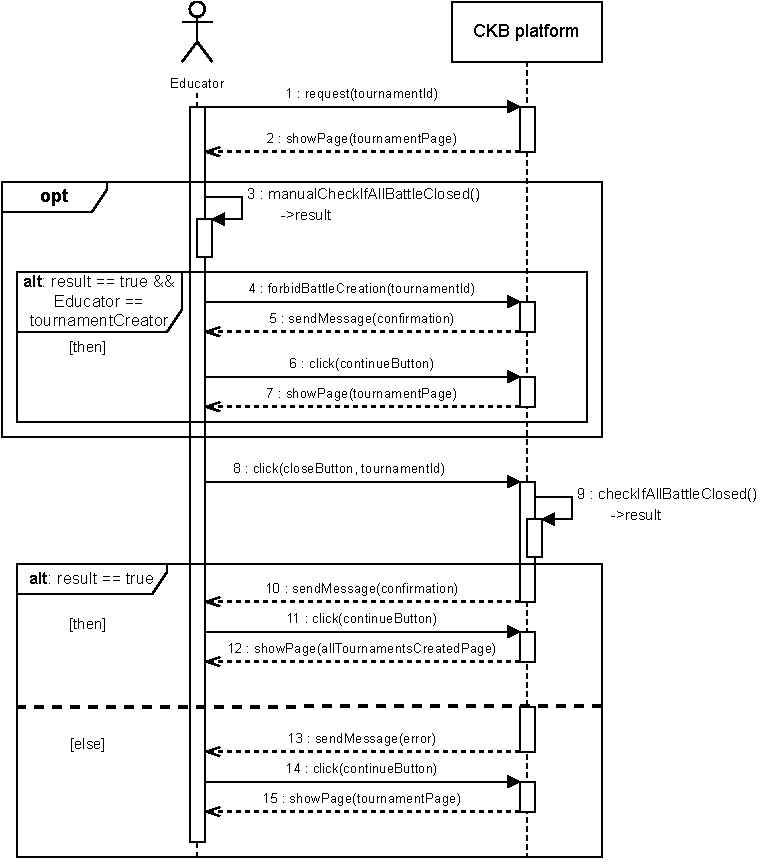
\includegraphics[scale=0.95]{images/SequenceDiagrams/Sequence7.pdf}
              \caption{Educator closes a tournament sequence diagram}
              \label{fig:TournamentClosingSeqDiagram}
          \end{figure}

    \newpage
    \item[\textbf{8.}] \textbf{Educator evaluates a battle's results}
          \begin{xltabular}{\textwidth}
              {| >{\raggedright\arraybackslash}g | >{\raggedright\arraybackslash}X |}
              \hline
              \endfirsthead
              \hline
              \endhead
              \endfoot
              \hline
              \endlastfoot




              \textbf{Name} & Battle's results evaluation\\
              \hline
              \textbf{ID} & UC.8\\
              \hline
              \textbf{Actors} & Educator\\
              \hline
              \textbf{Entry condition} & Educator has logged in the platform, has created at least one battle
              within a tournament that has terminated. Educator wants to manually evaluate the results\\
              \hline
              \textbf{Flow of events} &    \begin{enumerate}
                  \item[1.] Educator accesses the page related to the tournament
                        he has created.
                  \item[2.] Educator accesses the page related to a terminated
                        battle within that tournament and that is in the consolidation phase.
                  \item[3.] Educator manually evaluates groups' works by decreasing or
                        increasing their scores according to his personal preferences or
                        the ones accorded with the students.
                  \item[4.] Educator after evaluating all the groups proceeds to
                        definitively close the battle.
              \end{enumerate} \\
              \hline
              \textbf{Exit condition} & Groups' scores within the battle get updated by the platform,
              battle is definitively closed and the Educator is led back to the riepilogative page of
              the tournament whom the battle belonged.\\
              \hline
              \textbf{Exceptions} &    \begin{itemize}
                  \item[2.1] The battle cannot be manually evaluated.
                  \item[2.2] Accessed battle isn't terminated.
                        \begin{itemize}
                            \item[$\rightarrow$] CKB platform doesn't allow the Educator to manually evaluate
                                  the battle. Flow restarts from point 2.
                        \end{itemize}
              \end{itemize}
          \end{xltabular}

          \begin{figure}[H]
              \centering
              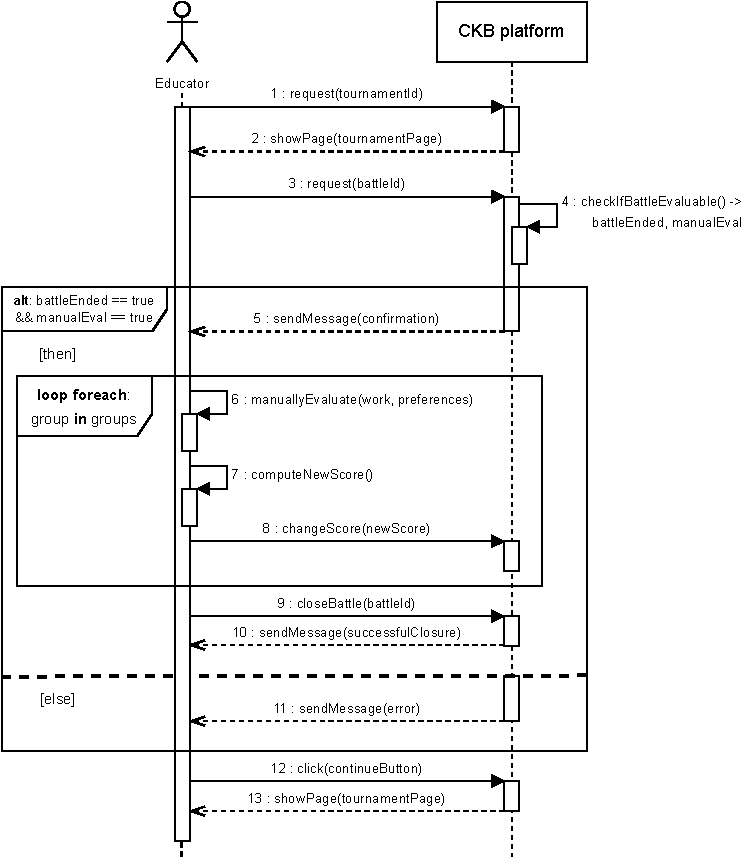
\includegraphics[scale=0.95]{images/SequenceDiagrams/Sequence8.pdf}
              \caption{Educator evaluates manually a battle's score sequence diagram}
              \label{fig:BattleEvalSeqDiagram}
          \end{figure}

    \newpage
    \item[\textbf{9.}] \textbf{Student forms a group}
          \begin{xltabular}{\textwidth}
              {| >{\raggedright\arraybackslash}g | >{\raggedright\arraybackslash}X |}
              \hline
              \endfirsthead
              \hline
              \endhead
              \endfoot
              \hline
              \endlastfoot




              \textbf{Name} & Group formation\\
              \hline
              \textbf{ID} & UC.9\\
              \hline
              \textbf{Actors} & Student\\
              \hline
              \textbf{Entry condition} & Student has logged in the platform, has subscribed to a
              tournament and wants to form a group in order to later join a battle within that
              tournament.\\
              \hline
              \textbf{Flow of events} &    \begin{enumerate}
                  \item[1.] Student clicks on a button that leads to
                        an appropriate page to form a group between Students.
                  \item[2.] Student choose the filters to search one or more
                        other Students to invite.
                  \item[3.] CKB platform computes all the filters and returns to
                        the Student the available Students, according to the filters he inserted.
                  \item[4.] Student chooses the other Students to whom send
                        the invite from the showed page.
                  \item[5.] Student clicks on confirm button to send the invitations.
                  \item[6.] CKB platform proceeds to send the invitations to all Students
                        specified and sends a notification with it in order to notify the receivers.
                  \item[7.] Invited Students accept the invitation.
                  \item[8.] CKB platform sends notification to the Student.
              \end{enumerate} \\
              \hline
              \textbf{Exit condition} & The group is formed and registered by the
              CKB platform. The Student is led back to the tournament's riepilogative page.\\
              \hline
              \textbf{Exceptions} &    \begin{itemize}
                  \item[3.1] The set of Students returned applying the filters
                        doesn't contain any available Student.
                        \begin{itemize}
                            \item[$\rightarrow$] CKB platform shows an empty list, with
                                  a message explaining the absence of Students in the list. Flow restarts from point 2.
                        \end{itemize}
                  \item[3.2] The set of Students returned contains only Students
                        already in a group.
                        \begin{itemize}
                            \item[$\rightarrow$] CKB platform shows the Students returned
                                  from the computation but doesn't allow the Student to select them.
                                  Flow restart from point 2.
                        \end{itemize}
                  \item[7.1] One or more invited Students don't accept the invitation
                        \begin{itemize}
                            \item[$\rightarrow$] CKB platform notifies the Student that sent the invitation
                                  of the received refusal. Flow restarts from point 1.
                        \end{itemize}
              \end{itemize}
          \end{xltabular}

          \begin{figure}[H]
              \centering
              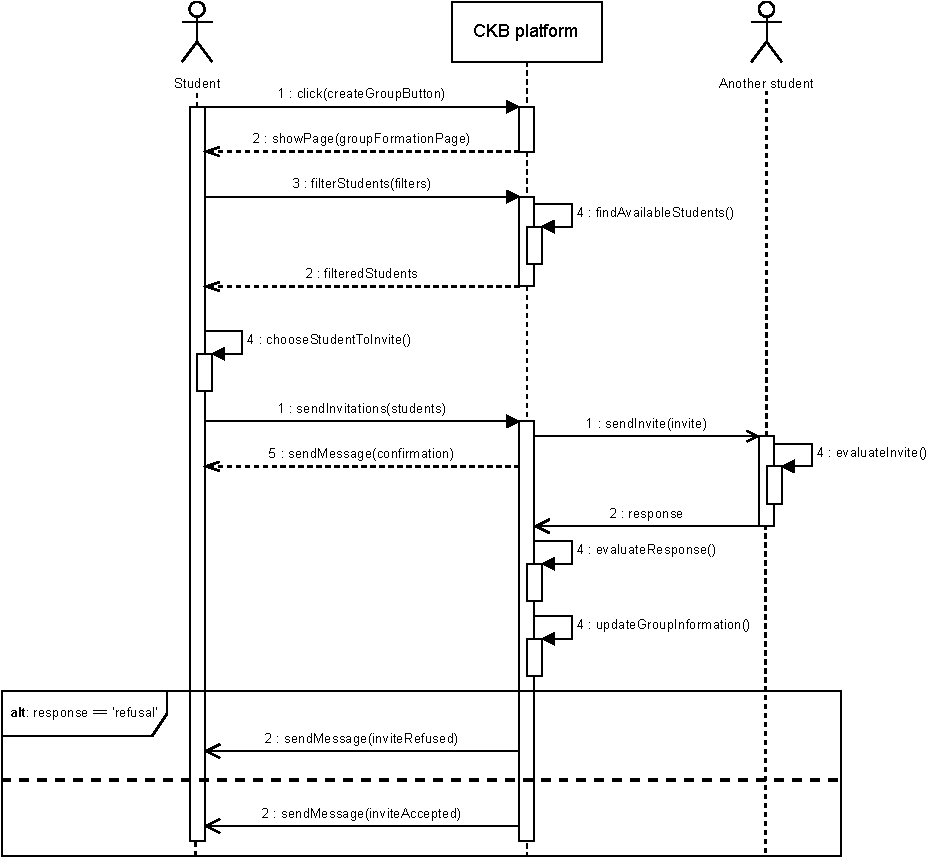
\includegraphics[scale=0.95]{images/SequenceDiagrams/Sequence9.pdf}
              \caption{Students form a new group sequence diagram}
              \label{fig:GroupFormationSeqDiagram}
          \end{figure}

    \newpage
    \item[\textbf{10.}] \textbf{Student joins a battle}
          \begin{xltabular}{\textwidth}
              {| >{\raggedright\arraybackslash}g | >{\raggedright\arraybackslash}X |}
              \hline
              \endfirsthead
              \hline
              \endhead
              \endfoot
              \hline
              \endlastfoot




              \textbf{Name} & Battle joining\\
              \hline
              \textbf{ID} & UC.10\\
              \hline
              \textbf{Actors} & Student\\
              \hline
              \textbf{Entry condition} & Student has logged in the platform, has subscribed to a
              tournament and wants to join a battle within that tournament.\\
              \hline
              \textbf{Flow of events} &    \begin{enumerate}
                  \item[1.] Student enters the tournament's page and
                        subsequently the battle's page.
                  \item[2.] Student clicks on the button to join the battle.
                  \item[3.] CKB platform shows a riepilogative page of
                        the battle.
                  \item[4.] Student clicks on the button to subscribe his group 
                        to the battle.
                  \item[5.] CKB platform checks whether the group respects all of the
                        battle requirements.
                  \item[5.] CKB platform returns a confirmation message to all the group
                        members.
                  \item[6.] CKB platform sends a notification to the group members
                        when the subscription deadline expires and battle starts.
              \end{enumerate} \\
              \hline
              \textbf{Exit condition} & The Student and his group have joined the battle.
              CKB platform starts saving all the solutions and statistics regarding the group's
              work. The Student is led to the riepilogative page of the battle.\\
              \hline
              \textbf{Exceptions} &    \begin{itemize}
                  \item[5.1] The group doesn't respect the battle's requirements
                        (too many or too few members).
                  \item[5.2] The group contains members not subscribed to the tournament in which
                        the battle is held.
                        \begin{itemize}
                            \item[$\rightarrow$] CKB platform shows an error message.
                        \end{itemize}
              \end{itemize}
          \end{xltabular}

          \begin{figure}[H]
              \centering
              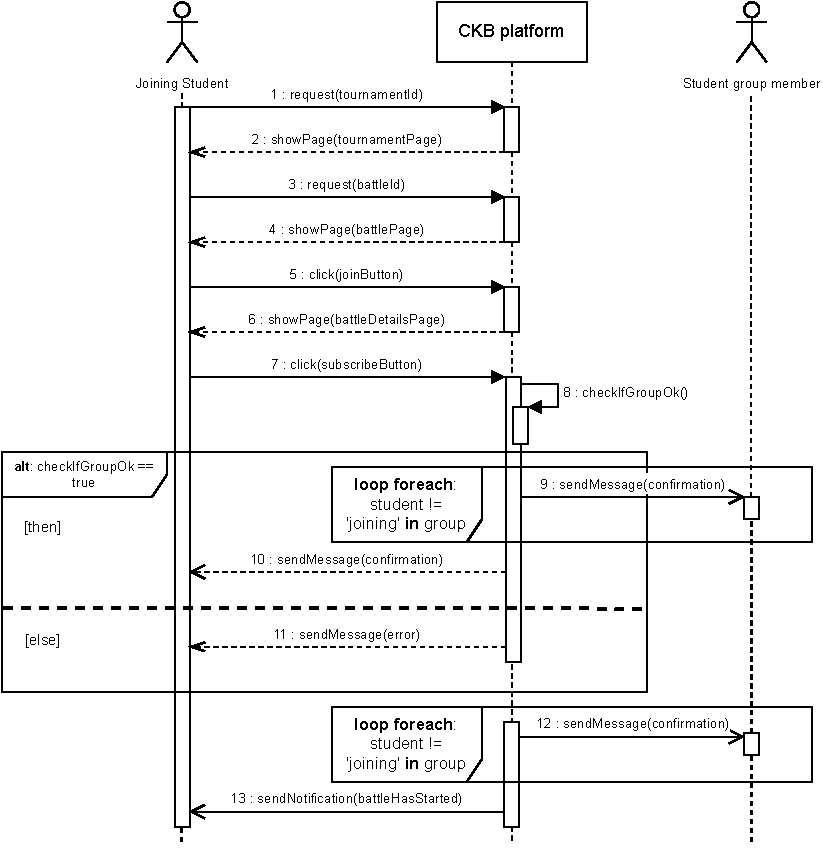
\includegraphics[scale=0.95]{images/SequenceDiagrams/Sequence10.pdf}
              \caption{Student joins a battle within a tournament, sequence diagram}
              \label{fig:BattleJoiningSeqDiagram}
          \end{figure}

    \newpage
    \item[\textbf{11.}] \textbf{Student uploads a new solution}
          \begin{xltabular}{\textwidth}
              {| >{\raggedright\arraybackslash}g | >{\raggedright\arraybackslash}X |}
              \hline
              \endfirsthead
              \hline
              \endhead
              \endfoot
              \hline
              \endlastfoot




              \textbf{Name} & Upload of a solution within deadline\\
              \hline
              \textbf{ID} & UC.11\\
              \hline
              \textbf{Actors} & Student, GitHub\\
              \hline
              \textbf{Entry condition} & Student has a GitHub account, has registered to at least one tournament
              and one battle in it, and wants to upload a new solution to that battle. \\
              \hline
              \textbf{Flow of events} &    \begin{enumerate}
                  \item[1.] Student accesses his GitHub account.
                  \item[2.] Student uploads group's solution
                        to his GitHub repository, precedently forked.
                  \item[3.] GitHub platform, through its "GitHub Actions" notifies
                        the CKB platform of the upload of the new solution by the Student.
                  \item[4.] CKB platform receives the new solution uploaded and starts
                        testing it.
                  \item[5.] CKB platform gives a score to the solution based on the
                        tests' results.
                  \item[6.] CKB platform updates the group's score in the battle and tournament.
                  \item[7.] CKB platform notifies the group's members of the successful testing.
              \end{enumerate} \\
              \hline
              \textbf{Exit condition} & Student's (or his group's) score is updated based on the
              uploaded solution.
              \\
              \hline
              \textbf{Exceptions} &    \begin{itemize}
                  \item[2.1] Generic upload error.
                        \begin{itemize}
                            \item[$\rightarrow$] Handled by GitHub, flow restarts from point 2.
                        \end{itemize}
                  \item[4.1] Tested code generated major issues, such as infinite loops,
                        huge resources consumption, ...
                        \begin{itemize}
                            \item[$\rightarrow$] CKB platform terminates the testing phase and
                                  notifies the Student's group with an error message instead of the
                                  solution score, flow ends.
                        \end{itemize}
              \end{itemize}
          \end{xltabular}

          \begin{figure}[H]
              \centering
              \hspace*{-1.6cm}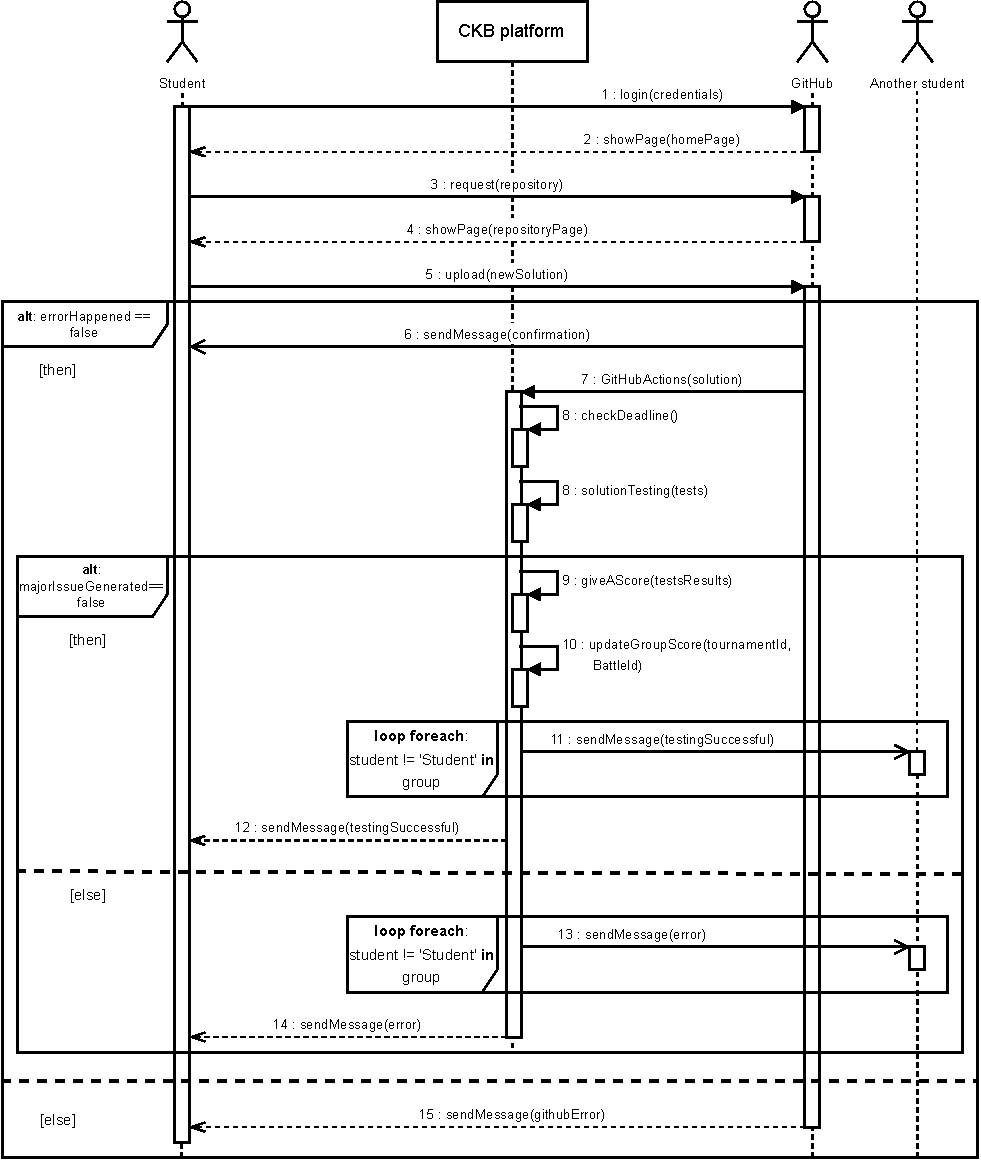
\includegraphics[scale=0.92]{images/SequenceDiagrams/Sequence11.pdf}
              \caption{Student uploads a new solution of the battle's problem within the deadline, sequence diagram}
              \label{fig:CorrectSolutionUploadSeqDiagram}
          \end{figure}

    \item[\textbf{12.}] \textbf{Student uploads a solution after submission deadline}
          \begin{xltabular}{\textwidth}
              {| >{\raggedright\arraybackslash}g | >{\raggedright\arraybackslash}X |}
              \hline
              \endfirsthead
              \hline
              \endhead
              \endfoot
              \hline
              \endlastfoot




              \textbf{Name} & Solution upload exceeding deadline\\
              \hline
              \textbf{ID} & UC.12\\
              \hline
              \textbf{Actors} & Student\\
              \hline
              \textbf{Entry condition} & Student has logged in the platform, has registered to at least one tournament
              and one battle within it, and wants to upload a new solution to that battle, but the submission deadline
              expired. \\
              \hline
              \textbf{Flow of events} &    \begin{enumerate}
                  \item[1.] Student accesses his GitHub account.
                  \item[2.] Student uploads his solution
                        to the group's GitHub repository, precedently forked.
                  \item[3.] GitHub platform, through his "GitHub Actions" notifies
                        the CKB platform of the Student's new solution's upload.
                  \item[4.] CKB platform receives the new solution uploaded and sees
                        that the submission deadline of the battle for which the solution
                        was uploaded has expired.
                  \item[5.] CKB platform notifies the group's members of the error by sending an error message.
              \end{enumerate} \\
              \hline
              \textbf{Exit condition} & Student's (or his group's) receives a notification by the CKB platform
              stating that their last uploaded solution will not be considered on the final score since the
              submission deadline has expired.\\
              \hline
              \textbf{Exceptions} &    \begin{itemize}
                  \item[2.1] Generic upload error.
                        \begin{itemize}
                            \item[$\rightarrow$] Handled by GitHub, flow restarts from point 2.
                        \end{itemize}
              \end{itemize}
          \end{xltabular}

          \begin{figure}[H]
              \centering
              \hspace*{-2cm}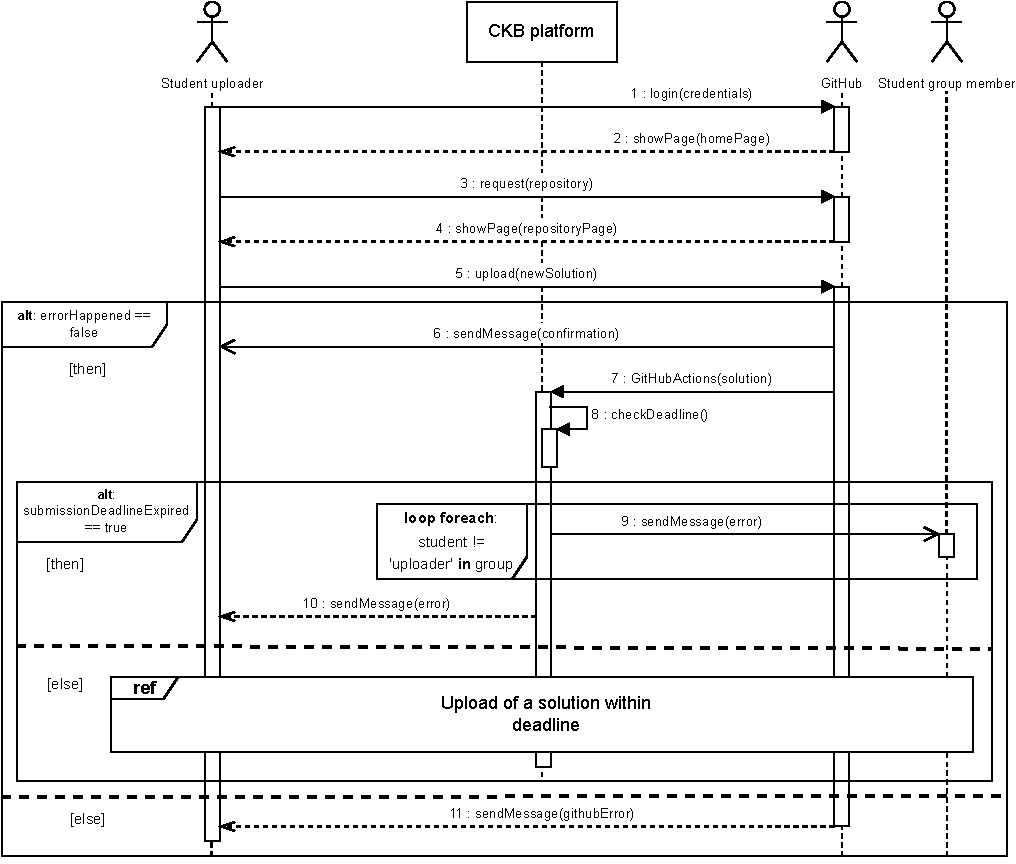
\includegraphics[scale=0.95]{images/SequenceDiagrams/Sequence12.pdf}
              \caption{Student uploads a solution after submission deadline sequence diagram}
              \label{fig:WrongSolutionUploadSeqDiagram}
          \end{figure}

    \newpage
    \item[\textbf{13.}] \textbf{Student visualises his tournament's results and badges}
          \begin{xltabular}{\textwidth}
              {| >{\raggedright\arraybackslash}g | >{\raggedright\arraybackslash}X |}
              \hline
              \endfirsthead
              \hline
              \endhead
              \endfoot
              \hline
              \endlastfoot




              \textbf{Name} & Viewing results and badges \\
              \hline
              \textbf{ID} & UC.13\\
              \hline
              \textbf{Actors} & Student\\
              \hline
              \textbf{Entry condition} & Student has logged in the platform and wants to
              see his or others' tournament's scores and badges.\\
              \hline
              \textbf{Flow of events} &    \begin{enumerate}
                  \item[1.] Student enters in his profile page or in the profile
                        page of the Student he wants to see the tournament scores
                        and badges.
                  \item[2.] Student chooses the tournament of which he wants to see the
                        details from the appropriate section.
                  \item[3.] Student consults his tournament scores and badges
              \end{enumerate} \\
              \hline
              \textbf{Exit condition} & Student has consulted his tournament score and badges obtained
              during it. The Student can see several details about all the tournaments
              in which he partecipated. Flow ends when the Student goes back to a precedent page.
              \\
              \hline
              \textbf{Exceptions} &    \begin{itemize}
                  \item[2.1] The Student has not yet participated in any tournament.
                        \begin{itemize}
                            \item[$\rightarrow$] CKB platform still allows the Student to
                                  access the profile page of the Student that hasn't partecipated
                                  to any tournament, but doesn't show anything regarding tournaments.
                                  Flow ends.
                        \end{itemize}
              \end{itemize}
          \end{xltabular}

          \begin{figure}[H]
              \centering
              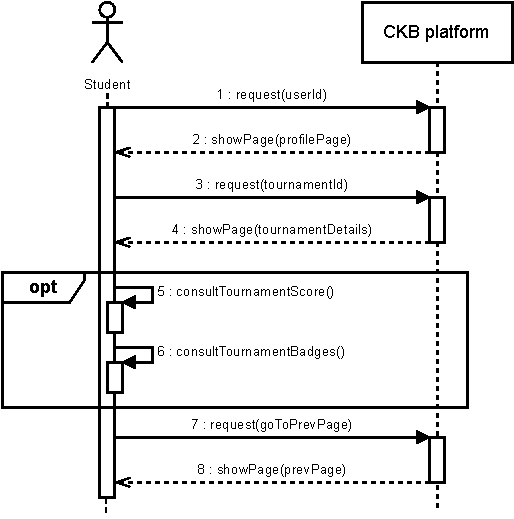
\includegraphics[scale=0.95]{images/SequenceDiagrams/Sequence13.pdf}
              \caption{Student visualises his/other score(s) and badge(s), sequence diagram}
              \label{fig:ScoresBadgesVisualizationSeqDiagram}
          \end{figure}
\end{enumerate}

\newpage
\subsubsection{Traceability matrix}
\begin{xltabular}{\textwidth}
    {| >{\raggedright\arraybackslash}g | >{\raggedright\arraybackslash}X | >{\raggedright\arraybackslash}X | >{\raggedright\arraybackslash}X |}
    \hline
    \endfirsthead
    \hline
    \endhead
    \endfoot
    \hline
    \endlastfoot

    \textbf{Goal ID} & \multicolumn{1}{|g|}{\textbf{Req. ID}} & \multicolumn{1}{|g|}{\textbf{Use case ID}} & \multicolumn{1}{|g|}{\textbf{Assump. ID}} \\
    \hline
    \textbf{G.1} & R.2, R.3, R.5, R.6, R.8, R.10, R.12, R.14, R.15, R.16, R.17, R.18 & UC.2, UC.3, UC.4, UC.5 & D.1, D.2, D.3, D.8, D.9, D.15\\
    \textbf{G.2} & R.2, R.3, R.5, R.6, R.8, R.9, R.11, R.40 & UC.2, UC.6 & D.1, D.2, D.3, D.9, D.11, D.15\\
    \textbf{G.3} & R.2, R.3, R.5, R.6, R.19, R.20 & UC.2, UC.7 & D.1, D.2, D.3, D.13, D.15\\
    \textbf{G.4} & R.2, R.3, R.5, R.6, R.13, R.34 & UC.2, UC.8 & D.1, D.2, D.3, D.12, D.15\\
    \textbf{G.5} & R.1, R.3, R.4, R.7, R.24 & UC.1 & D.1, D.2, D.3, D.9, D.15\\
    \textbf{G.6} & R.1, R.3, R.4, R.7, R.25, R.27, R.28 & UC.1, UC.10 & D.1, D.2, D.3, D.4, D.5, D.6, D.9, D.14, D.15\\
    \textbf{G.6.1} & R.1, R.3, R.4, R.7, R.27 & UC.1, UC.9 & D.1, D.2, D.3, D.14, D.15, D.16\\
    \textbf{G.6.2} & R.1, R.3, R.4, R.7, R.21, R.26, R.29, R.30, R.31, R.32 & UC.1, UC.11, UC.12 & D.1, D.2, D.3, D.4, D.5, D.7, D.9, D.10, D.15\\
    \textbf{G.6.3} & R.1, R.3, R.4, R.7, R.22, R.23, R.33, R.37, R.38, R.39 & UC.1, UC.13 & D.1, D.2, D.3, D.12, D.15\\
    \textbf{G.7} & R.1, R.3, R.4, R.7, R.35, R.36 & UC.1, UC.3, UC.6 & D.1, D.2, D.3, D.15\\

\end{xltabular}
\subsection{Performance requirements}
We expect thousands of registrations to the platform, due to the possible
subscription of several private and public academic environments (especially high schools).
In the subsequent years we expect to have way less subscriptions, since the first year every school and university student
will have the need to subscribe to the platform.
After this first boom of subscriptions, in the subsequent years only new students will have to subscribe, hence there is no need to 
have such a high tolerance in scalability.
There is also to consider the fact that not many people will access the platform at the same time, since once a Student has subscribed 
to a battle, he can work locally and only interact with the GitHub platform.
We expect the CKB platform to be accessed only when a new tournament or battle is created, and when a tournament or a battle is closed,
so that Students can access the platform and check their results. Response time and reliability are our main focuses.
We need to guarantee a low response time in order to let Students and Educators interact actively with the platform
without high delays that could compromise Students' works.
We have to take into consideration reliability since with a low reliability platform when Students upload their solutions on the
forked GitHub repository, triggering GitHub Actions to upload the solutions to the CKB platform, if the CKB platform is not reliable,
it could cause delays in the solution's uploading to the platform.
A low reliable platform can also mean that Student's solutions may not be correctly graded, since the platform may incur in a byzantine failure
type and erroneusly attributes points to some solutions.
Educators would also not be able to access the platform and manually evaluate Students' solutions, and would be a bad experience overall.
For data storing, we expect we'll need a high capacity DB. It's necessary for storing
the user's data, tournaments and battles' data and statistics, informations and code about groups' commits.
We'll need a high capacity DB, since being the platform built around students and schools, we expect to have lots of users subscribing together
at the same time, when school starts. These times are differenciated throught the year, for example in Italy schools starts in Semptember, while in
New Zealand it starts in July. The platform being based around schools means that we'll have lots of user's data related to old students that are
 now not using the platform anymore.
\subsection{Design constraints}
\subsubsection{Hardware constraints}
The users, both Educators and Students, to have access to the platform need to have a functioning internet access and a device connected to the net.
The Educators must have at least a smartphone, so that they can perform all of the different functions the platform offers them, like creating new battles
and tournament, badges and manually evaluate groups' solutions. All of this can be done via browser installed on a smartphone.
The Students are required to have a personal computer, either a desktop or a laptop, such that they can write and submit their solutions to the platform.
Students can access the platform via smartphone too, for consulting their profile and looking at new tournaments and battles, but it would be
best if everything that is concerning to coding and submitting a solution is done via personal computer.
\subsubsection{Privacy constraints}
Since the main application area is the european one, the platform must be compliant to the GDPR's law.
Data must be encrypted before it is saved on the DB, no data must be accessed by any user other than the data's owner.
For preventing cyber attacks, data must pass through secure connections and channels. In this case, no \textit{Man in the Middle} attacks can occur.
Autentication and login will be provided by the CKB platform, so all data must be treated accordingly to the platform's privacy policy.
When a new User, both Educator and Student, wants to register to the platform, the privacy policy must be shown and 
accepted, before the new user is saved in the DB.
If the privacy policy is not accepted, the user registration procedure is not completed and
 the new user is not saved in the DB, not granting access to the person that was
trying to register to the platform.
\subsection{Software system attributes}
\subsubsection{Usability}
The platform must be easy to use. Users must not have doubts on which page to go to perform a precise task.
Each button and link must be named accordingly, to limit time waste and useless interaction with the platform.
\subsubsection{Reliability}
The platform must prevent downtime in order to notify Students of new tournaments or battles as soon as they are created, in order to let
Educators create new tournaments and battles whenever they want and for correctly publish new evaluations and grades on the platform for
Students to see and access.
We expect the highest number of simultaneous access to be whenever schools start and end, since more students will register on school starting,
and more will rush to finish battles and projects as school is ending.
\subsubsection{Availability}
The platform must be available as much as possible, at least 99\% of the time.
Both Students and Educators must have access to the platform whenever they need to.
\subsubsection{Security}
Communication between Users and the Platform must pass through secure channels, and it must be encrypted.
With a web certificate for the platform we can ensure that the SSL protocol is followed, and can ensure security for the platform and its Users.
The DB guarantees that performed operations are all authorized, and permitted.
\textit{A Student cannot create new battles, for example.}
\subsubsection{Web Browsing}
The platform must be usable on any major web browser, since access to it is fully online.
\subsubsection{Maintainability}
The platform must be designed in a way that eases the future adding of new features with the least possible effort.
Maintainability is also key for having a functioning platform, since the easier it is to maintain, the easier errors, 
reliability and availability failures can be corrected.
\newpage
\pagestyle{FormalAnalysisAlloyStyle}

\section{Formal analysis using Alloy}

\subsection{Signatures}
\color{gray}
//Used to represent an Educator subscribed to the CBK platform \\
\color{blue}
sig
\color{black}
Educator  \{\} \\
\\
\color{gray}
//A Permit is given by an Educator to a set of other Educators, and regards only one tournament created by the permit's sender\\
\color{blue}
sig
\color{black}
Permit \{\\
\-\hspace{1cm}    tournamentCreator : \color{blue} one \color{black} Educator,\\
\-\hspace{1cm}    battleCreators : \color{blue} some \color{black} Educator,\\
\-\hspace{1cm}    tournament : \color{blue} one \color{black} Tournament\\
\}	\{\\
\-\hspace{1cm}    tournamentCreator \color{blue} not in \color{black} battleCreators \color{blue} and \color{black}\\
\-\hspace{1cm}    tournament.creator \color{blue} = \color{black} tournamentCreator \color{blue} and \color{black}\\
\-\hspace{1cm}    tournament.battleCreators \color{blue} = \color{black} battleCreators\\
\}\\
\\
\color{gray}
//A tournament has a creator and a set of Educators that can create battles in it\\
\color{blue}
sig
\color{black}
Tournament \{ \\
\-\hspace{1cm}    creator : \color{blue} one \color{black} Educator,\\
\-\hspace{1cm}    battleCreators : \color{blue} set \color{black} Educator\\
\}\\
\color{gray}
\\
//A battle has a creator and a tournament to which it belongs, the creator must be the tournament's creator or another Educator that can create battles within that tournament\\
\color{blue}
sig
\color{black}
Battle \{\\
\-\hspace{1cm}    tournament : \color{blue} one \color{black} Tournament,\\
\-\hspace{1cm}    creator : \color{blue} one \color{black} Educator,\\
\-\hspace{1cm}	tests : \color{blue} set \color{black} Test\\
\}\{\\
\-\hspace{1cm}	creator \color{blue} in \color{black} tournament.battleCreators \color{blue} or \color{black}\\
\-\hspace{1cm}	creator \color{blue} = \color{black} tournament.creator\\
\}\\
\color{gray}
\\
//Test represents a battle's test\\
\color{blue}
sig
\color{black}
Test \{\}

\newpage

\color{gray}
//Students subscribed to the CKB platform can have a set of badges\\
\color{blue}
sig
\color{black}
Student\{\\
\-\hspace{1cm}    badges : \color{blue} set \color{black} Badge,\\
\-\hspace{1cm}    tournament : \color{blue} set \color{black} Tournament\\
\}\\
\color{gray}
\\
//A repository is assigned to a group and is relative to one battle\\
\color{blue}
sig
\color{black}
Repository\{\\
\-\hspace{1cm}    group : \color{blue} one \color{black} Group,\\
\-\hspace{1cm}    battle : \color{blue} one \color{black} Battle\\
\}\{\\
\-\hspace{1cm}    group.battle \color{blue} = \color{black} battle\\
\}\\
\\
\color{gray}
//A group is formed by some Students and partecipates to one battle\\
\color{blue}
sig
\color{black}
Group\{\\
\-\hspace{1cm}    groupCreator : \color{blue} one \color{black} Student,\\
\-\hspace{1cm}    students : \color{blue} set \color{black} Student,\\
\-\hspace{1cm}    battle : \color{blue} lone \color{black} Battle\\
\}\{\\
\-\hspace{1cm}    groupCreator \color{blue} not in \color{black} students	\\
\}\\
\\
\color{gray}
//A badge is created by an Educator\\
\color{blue}
sig
\color{black}
Badge\{\\
\-\hspace{1cm}    creator : \color{blue} one \color{black} Educator,\\
\-\hspace{1cm}    tournament : \color{blue} one \color{black} Tournament\\
\}\{\\
\-\hspace{1cm}    creator \color{blue} = \color{black} tournament.creator\\
\}\\
\\
\color{gray}
//An invite is made by a Student of a group and directed to another Student\\
\color{blue}
sig
\color{black}
Invite\{\\
\-\hspace{1cm}    sender : \color{blue} one \color{black} Student,\\
\-\hspace{1cm}    receiver : \color{blue} one \color{black} Student,\\
\-\hspace{1cm}    group : \color{blue} one \color{black} Group\\
\}\{\\
\-\hspace{1cm}    sender \color{blue} != \color{black} receiver \color{blue} and \color{black}\\
\-\hspace{1cm}    sender \color{blue} = \color{black} group.groupCreator \\
\}\\
\\
\color{gray}
//Signature that defines the state of the battle\\
\color{blue} abstract sig \color{black} BattleState{}\\
\\
\color{blue} one sig \color{black}  RegistrationPhase \color{blue} extends \color{black} BattleState{}\\
\color{blue} one sig \color{black}  SubmissionPhase \color{blue} extends \color{black} BattleState{}\\
\color{blue} one sig \color{black}  ConsolidationPhase \color{blue} extends \color{black} BattleState{}\\
\color{blue} one sig \color{black}  ClosedBattle \color{blue} extends \color{black} BattleState{}\\
\\
\color{gray}
//Signature that defines the state of the invite\\
\color{blue} abstract sig \color{black} InviteState{}\\
\\
\color{blue} one sig \color{black} Accepted \color{blue} extends \color{black} InviteState{}\\
\color{blue} one sig \color{black} Refused \color{blue} extends \color{black} InviteState{}\\
\color{blue} one sig \color{black} Waiting \color{blue} extends \color{black} InviteState{}\\
\\
\subsection{Facts}
\color{gray}
//A tournament's creator can grant to (only once per Educator) another Educator the permission to create battles in his tournament\\
\color{black}
\color{blue} fact \color{black} NoTwoPermissionAtSameEducator\{\\
\-\hspace{1cm} \color{blue} all disj \color{black} p1, p2 : Permit | \\
\-\hspace{1cm} (p1.tournament \color{blue} = \color{black} p2.tournament an\color{blue} and \color{black}d p1.tournamentCreator \color{blue} = \color{black} p2.tournamentCreator) \\
\-\hspace{1cm} implies (\color{blue} all \color{black} bC : p1.battleCreators | bC \color{blue} not in \color{black} p2.battleCreators)\\
\}
\\
\color{gray}
//A group can have at most one repository for each battle\\
\color{blue} fact \color{black} onlyOneRepository \{\\
\-\hspace{1cm} \color{blue} all disj \color{black} r1, r2 : Repository | \color{blue} all \color{black} g : r1.group | \color{blue} all \color{black} b : r1.battle | \\
\-\hspace{1cm}b \color{blue} != \color{black} r2.battle or \\
\-\hspace{1cm}g \color{blue} != \color{black} r2.group \\
\}
\\
\color{gray}
//For each battle, a Student can participate to it while being in only one group\\
\color{black}
\color{blue} fact \color{black} noStudentsInMoreGroupInABattle\{\\
\-\hspace{1cm} \color{blue} all \color{black} s: Student | \color{blue} all disj \color{black} g1, g2: Group | \\
\-\hspace{1cm}(s \color{blue} in \color{black} g1.students \color{blue} and \color{black} s \color{blue} in \color{black} g2.students ) \color{blue} implies \color{black} g1.battle != g2.battle \\
\}\\
\\
\color{gray}
//The sender and the receiver of a group invite must have at least one tournament subscription in common\\
\color{black}
\color{blue} fact \color{black} SenderAndReceiverInSameTournament\{\\
\-\hspace{1cm} \color{blue} all \color{black} i : Invite | \color{blue} all \color{black} r : i.receiver |  \color{blue} some \color{black} t : r.tournament | \\
\-\hspace{1cm} t \color{blue} in \color{black} i.sender.tournament \color{blue} and \color{black} i.inviteState = Accepted \\
\}\\
\\
\color{gray}
//All Students in a group must be subscribed to a tournament for the group to compete in one battle of that tournament\\%magic
\color{black}
\color{blue} fact \color{black} memberOfAGroupSameTournament\{\\
\-\hspace{1cm} \color{blue} all \color{black} g : Group | \color{blue} all disj \color{black} s1, s2 : g.students | \\
\-\hspace{1cm} \color{blue} some \color{black} t1 : s1.tournament | \color{blue} some \color{black} t2 : s2.tournament | \\
\-\hspace{1cm} t1 \color{blue} = \color{black} t2\\
\}\\
\\
\color{gray}
//Students must be subscribed to at least one battle to receive badges from it\\
\color{black}
\color{blue} fact \color{black} StudentReceiveBadges\{\\
\-\hspace{1cm} \color{blue} all \color{black} s:Student | \color{blue} all \color{black} b : s.badges | \color{blue} all \color{black} g: Group |  \\
\-\hspace{1cm} s \color{blue} in \color{black} g.students and    \\
\-\hspace{1cm} g.battle.tournament \color{blue} = \color{black} b.tournament\\
\}\\

\newpage
\color{gray}
//Students must be subscribed in a tournament to compete in that tournament's battles\\
\color{black}
\color{blue} fact \color{black} StudentsGroupBattleInTournament\{\\
\-\hspace{1cm} \color{blue} all \color{black} g : Group | \color{blue} all \color{black} s : g.students | \\
\-\hspace{1cm} g.battle.tournament \color{blue} in \color{black} s.tournament and \\
\-\hspace{1cm} g.battle.tournament \color{blue} in \color{black} g.groupCreator.tournament\\
\}\\
\\
\color{gray}
//A Student needs to receive at least one invite from the leader of a group to be a member of that group\\
\color{black}
\color{blue} fact \color{black} StudentInAGroup\{\\
\-\hspace{1cm} \color{blue} all \color{black} g : Group | \color{blue} all \color{black} s : g.students | \color{blue} some \color{black} i : Invite |\\
\-\hspace{1cm} i.sender \color{blue} = \color{black} g.groupCreator and\\
\-\hspace{1cm} i.receiver \color{blue} = \color{black} s  and \\
\-\hspace{1cm} i.group \color{blue} = \color{black} g\\
\}\\


\subsection{Examples of instances}
\begin{figure}[H]
    \centering
    \hspace*{-4.3cm}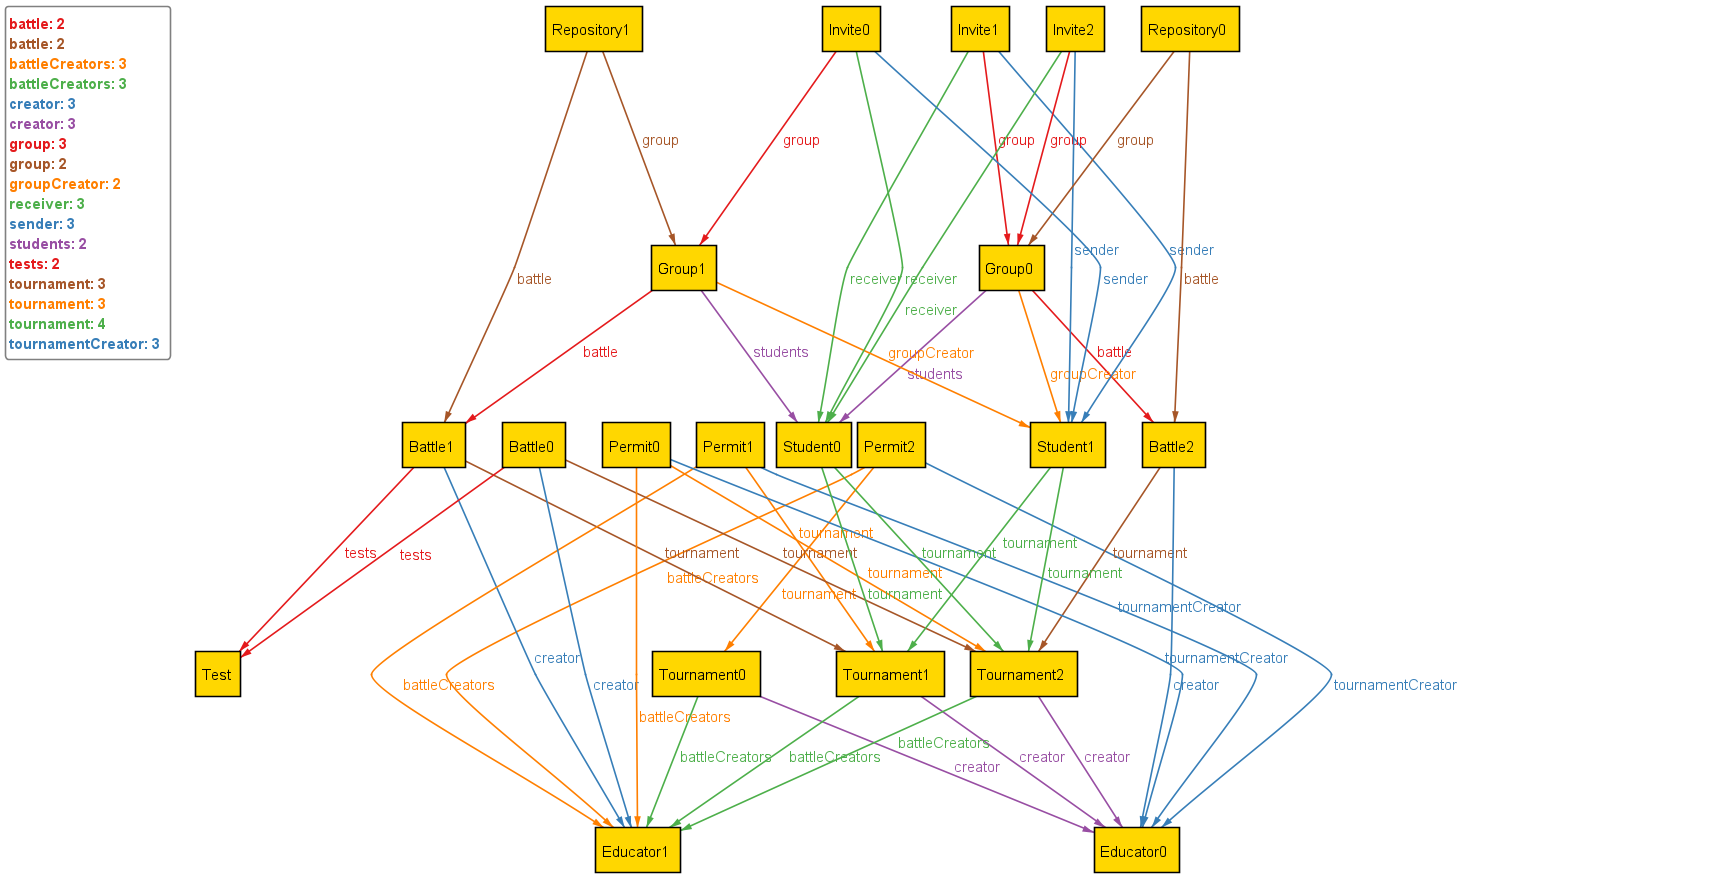
\includegraphics[scale=0.68]{images/ALLOY/AlloyInstance1.png}
    \caption{Picture of a general instance}
    \label{fig:Picture of a general instance}
\end{figure}
\begin{figure}[H]
    \centering
    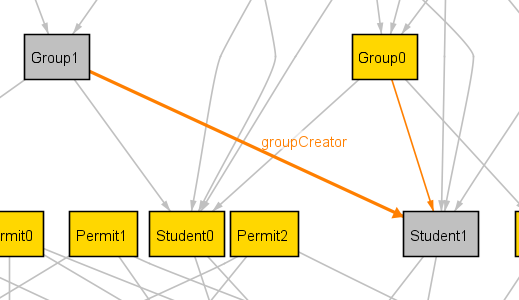
\includegraphics{images/ALLOY/groupCreator.png}
    \caption{Student1 have created Group0 and Group1}
    \label{fig:group creation}
\end{figure}
\begin{figure}[H]
    \centering
    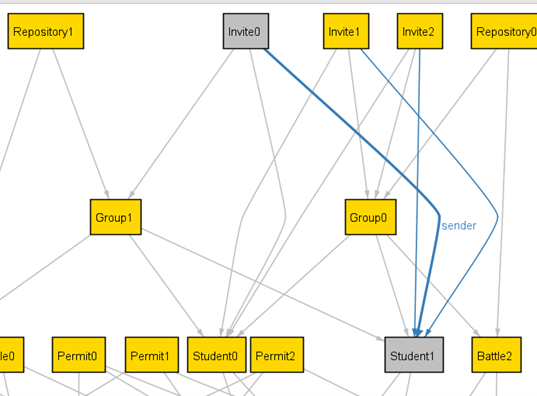
\includegraphics{images/ALLOY/sender.png}
    \caption{Student1 send 3 invite: Invite0, Invite1, Invite2}
    \label{fig:sending invite}
\end{figure}
\begin{figure}[H]
    \centering
    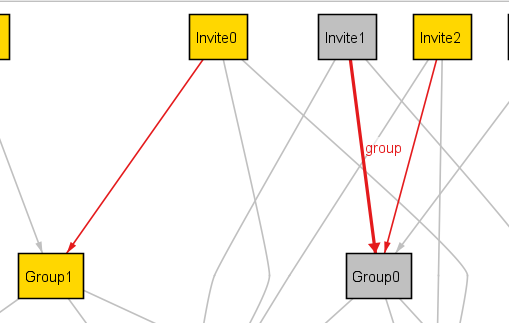
\includegraphics{images/ALLOY/group.png}
    \caption{Each invite is relative to one group}
    \label{fig:group invite}
\end{figure}
\begin{figure}[H]
    \centering
    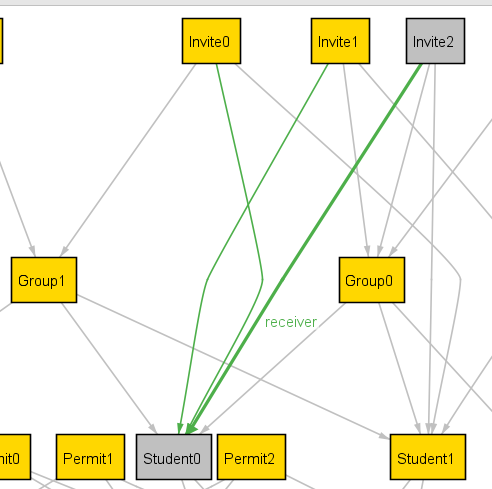
\includegraphics[scale=0.85]{images/ALLOY/receiver.png}
    \caption{All invite are being sent to Student0}
    \label{fig:receiving invite}
\end{figure}
\begin{figure}[H]
    \centering
    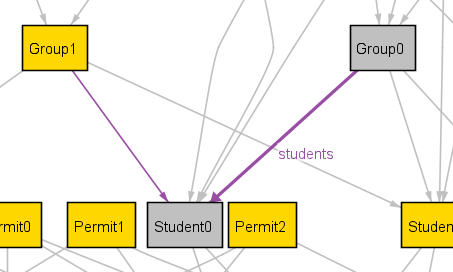
\includegraphics{images/ALLOY/students.png}
    \caption{Here we can see Student0 in group1 and group0, since he has received two invite for group0 he has rejected the first one but accepted the second one}
    \label{fig:receivingAcceptingRefusingInvite}
\end{figure}
\begin{figure}[H]
    \centering
    \hspace*{-4cm}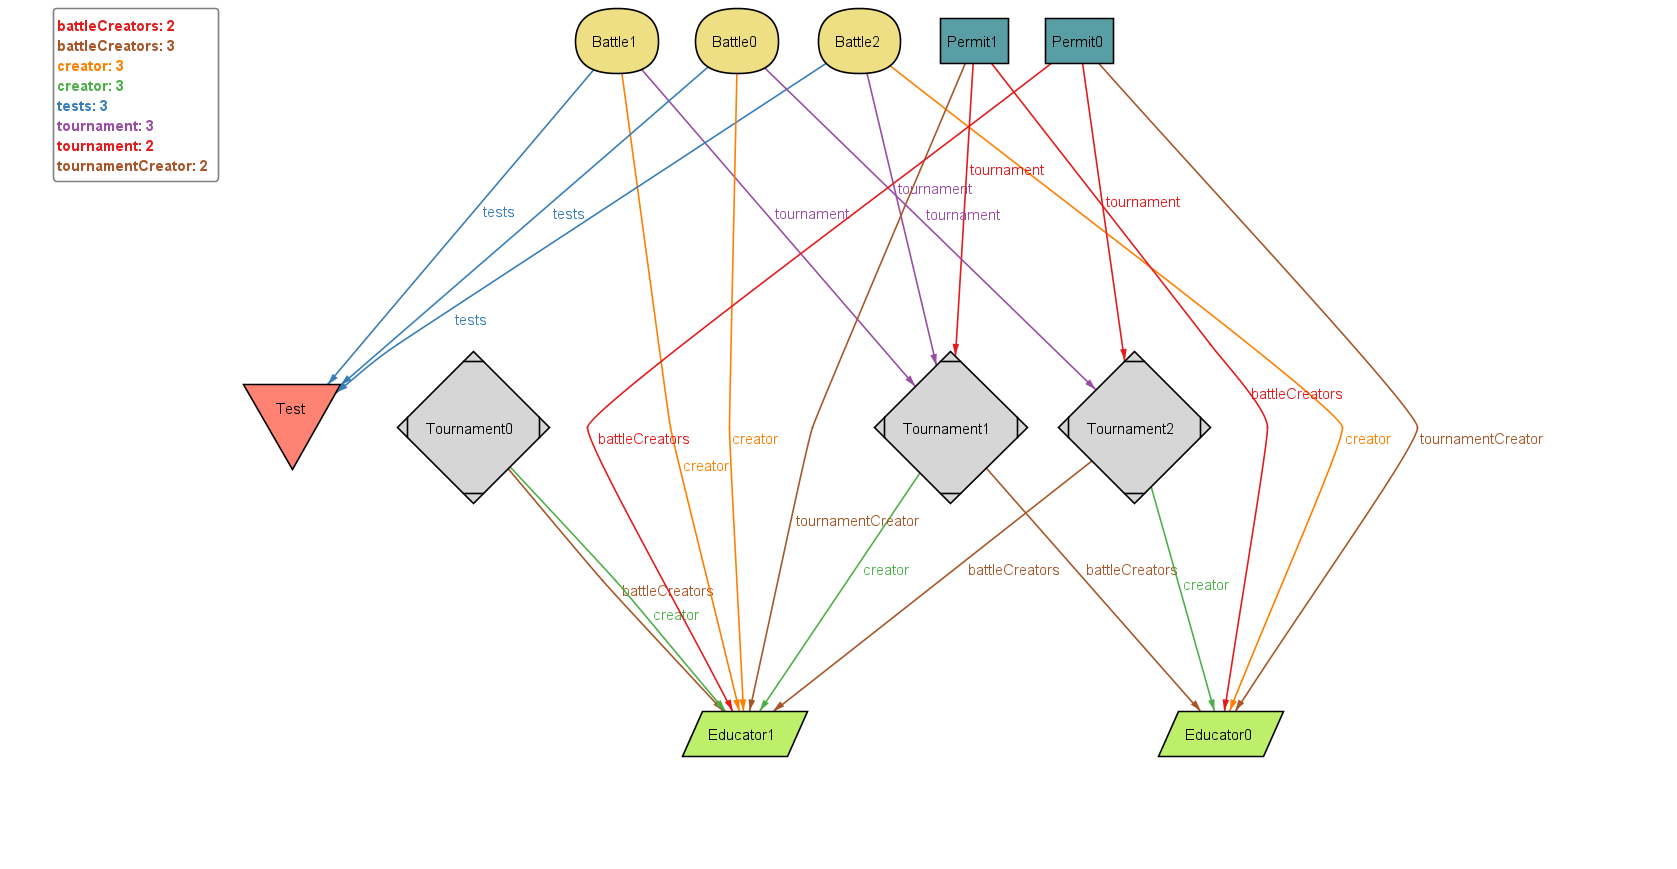
\includegraphics[scale=0.62]{images/ALLOY/AlloyTournament.png}
    \caption{tournament, educator and battle}
    \label{fig:tournament, Educator and battle}
\end{figure}
\color{red}
Every permit gives an Educator who isn't the creator, the possibility of creating new battles inside another Educator's tournament.
The tournament's creator must grant permission to the other Educator, via a permit. (battleCreators)\\
\color{orange}
Every battle is created by an Educator, he can be the tournament's creator or an Educator that has received 
modification permit by the tournament's creator (creator) [Ex. Battle0 is created by Educator1 in 
Tournament2, that is created by Educator0. Educator0 grants Educator1 Permit0 so that Educator1 can create Battle0 in Tournament2 ]\\
\color{green}
Every tournament can be created by only one Educator (creator)\\
\color{blue}
Tests may be reused amonst more battles, while a test has to be relative to at least one battle, it can be utilized by more than one (tests)\\
\color{violet}
A battle is only in one tournament (tournament)\\
\color{red}
A permission is relative to one tournament created by an Educator (tournament)\\
\color{brown}
A permission can only be granted by an Educator that created at least one tournament (tournamentCreator)\\
\color{black}

\pagestyle{EffortSpentStyle}

\section{Effort spent}
\begin{tabular}{|g|c|c|}
    \hline
    \multicolumn{2}{|g|}{\textbf{Group member}} & \multicolumn{1}{|g|}{\textbf{Effort spent}} \\
    \hline
    \textbf{Francesco Spangaro} & \makecell[l]{\\Introduction\\Overall description\\Specific Requirements\\Formal analysis using Alloy\\
     \vspace{\baselineskip}} & \makecell[l]{\textit{6h}\\\textit{14h}\\\textit{8h}\\\textit{2h} \vspace{\baselineskip}}\\
    \hline
    \textbf{Luca Tosetti} & \makecell[l]{\\Introduction\\Overall description\\Specific Requirements\\Formal analysis using Alloy\\
     \vspace{\baselineskip}} & \makecell[l]{\textit{6h}\\\textit{7h}\\\textit{19h}\\\textit{2h}}\\
    \hline
    \textbf{Francesco Riccardi} & \makecell[l]{\\Introduction\\Overall description\\Specific Requirements\\Formal analysis using Alloy\\
     \vspace{\baselineskip}} & \makecell[l]{\textit{6h}\\\textit{10h}\\\textit{2h}\\\textit{13h} \vspace{\baselineskip}}\\
    \hline
\end{tabular}

\newpage
\pagestyle{ReferencesStyle}

\section{References}
\subsection{Paper references}
\begin{itemize}
    \item Specification document Assignment RDD AY 2023-2024.pdf
    \item Alloy course's slides
\end{itemize}
\subsection{Used tools}
\begin{itemize}
    \item GitHub for project versioning.
    \item Diagrams.net for UML,Use case,Sequence and BPMN diagrams.
    \item Visual Studio Code as {\LaTeX} editor.
    \item Alloy analyzer for alloy code's formal analysis.
\end{itemize}

\end{document}
